\pdfoutput=1
\documentclass[twocolumn]{aastex61}
%%\documentclass[]{emulateapj}

%Accepted/received/... %%

\received{xxx}
\revised{yyy}
\accepted{zzz}

%% Command to document which AAS Journal the manuscript was submitted to.
\submitjournal{AAS Journals}

%% Short title/authors

\shorttitle{Tidal Torques in Stellar Binaries}
\shortauthors{Fleming et al.}

%% Begin document, title, packages %%
\usepackage{hyperref}
\usepackage{xspace}
\usepackage{graphicx}
\usepackage{amsmath}
\usepackage[caption=false]{subfig}

%% Custom commands
\def\mearth{{\rm\,M_\oplus}}
\def\rearth{{\rm\,R_\oplus}}
\def\msun{{\rm\,M_\odot}}
\def\rsun{{\rm\,R_\odot}}
\def\lsun{{\rm\,L_\odot}}
\def\gsim{~\rlap{$>$}{\lower 1.0ex\hbox{$\sim$}}}
\def\lsim{~\rlap{$<$}{\lower 1.0ex\hbox{$\sim$}}}

\newcommand{\vplanet}[0]{\texttt{VPLanet}\xspace}
\newcommand{\eqtide}[0]{\texttt{EQTIDE}\xspace}
\newcommand{\stellar}[0]{\texttt{STELLAR}\xspace}
\newcommand{\kepler}[0]{\textit{Kepler}\xspace}


%% Begin doc %%

\begin{document}

\title{Rotation Period Evolution in Low-Mass Binary Stars: The Impact of Tidal Torques and Magnetic Braking}

%% AUTHORS %%

%%\correspondingauthor{David P. Fleming}
%%\email{dflemin3@uw.edu}

%%\author[0000-0001-9293-4043]{David P. Fleming}
\author{David P. Fleming}
\affil{Astronomy Department, University of Washington \\
Box 951580, Seattle, WA 98195}
\affil{NASA Astrobiology Institute - Virtual Planetary Laboratory Lead Team, USA}

\author{Rory Barnes}
\affiliation{Astronomy Department, University of Washington \\
Box 951580, Seattle, WA 98195}
\affil{NASA Astrobiology Institute - Virtual Planetary Laboratory Lead Team, USA}

\author{James R. A. Davenport}
\affiliation{Astronomy Department, University of Washington \\
Box 951580, Seattle, WA 98195}

\author{Rodrigo Luger}
\affiliation{Center for Computational Astrophysics, Flatiron Institute \\
New York, NY 10010}
\affil{NASA Astrobiology Institute - Virtual Planetary Laboratory Lead Team, USA}

%% ABSTRACT %%

\begin{abstract}

Tidal torques dominate the angular momentum evolution of short-period, low-mass stellar binaries. Here we examine how tides, stellar evolution, and magnetic braking shape the rotation period (P$_{rot}$) evolution of low-mass stellar binaries out to orbital periods (P$_{orb}$) of 100 d across a wide range tidal dissipation parameters using two common equilibrium tidal models. We find that many binaries with P$_{orb} \lsim 20$ d tidally-lock, and most with $P_{orb} \lsim 4$ d tidally-lock into synchronous rotation on circularized orbits. At short P$_{orb}$, tidal torques produce a population of fast rotators that single-star only models of magnetic braking fail to produce.  In many cases, we show that the competition between magnetic braking and tides produces a population of subsynchronous rotators that persists for Gyrs, even in short P$_{orb}$ binaries, qualitatively reproducing the subsynchronous eclipsing binaries (EBs) discovered in the \kepler field by \citet{Lurie2017}. Both equilibrium tidal models predict that binaries can tidally-interact out to P$_{orb} \approx 80$ d, while the CPL equilibrium tidal model predicts that binaries can tidally-lock out to P$_{orb} \approx 100$ d. Tidal torques often force the P$_{rot}$ evolution of stellar binaries to depart from the long-term magnetic braking-driven spin down experienced by single stars, revealing that P$_{rot}$ is not be a valid proxy for age in all cases, i.e. gyrochronology methods can fail unless one accounts for binarity. We suggest that accurate determinations of orbital eccentricties and P$_{rot}$ can be used to discriminate between which equilibrium tidal models best describes tidal interactions in low-mass binary stars.

 %Tidal torques dominate the angular momentum evolution of short-period, low-mass stellar binaries. Here we examine how tides, stellar evolution, and magnetic braking shape the rotation period (P$_{rot}$) evolution of low-mass stellar binaries out to orbital periods (P$_{orb}$) of 100 d across a wide range tidal dissipation parameters. In many cases, we find that magnetic braking can overpower tides, producing a long-lasting population of subsynchronous rotators, even in short P$_{orb}$ binaries, reproducing the observed \kepler eclipsing binaries (EBs) population. Furthermore, at short P$_{orb}$, tidal locking naturally producing a population of fast rotators that cannot be reproduced by single-star-only models of magnetic braking.  Many binaries can tidally-lock even out to P$_{orb} \approx 100$ d, fixing P$_{rot}$ to P$_{orb}$, revealing that P$_{rot}$ is not be a valid proxy for age in all cases, i.e. gyrochronology methods must be applied carefully. We compare the predictions of two common equilibrium tidal models and show that the ``Constant Time Lag" equilibrium tidal model provides a better match to observations. We recommend observational tests to discriminate between which equilibrium tidal models best describes tidal interactions in low-mass binary stars. Finally, by comparing observations of \kepler EBs with our simulations, we constrain low-mass stellar tidal time lags to $\tau = 0.19^{+0.43}_{-0.16}$ s.

\end{abstract}

%% KEYWORDS %%

\keywords{binaries: close}

%% INTRO %%

\section{Introduction} \label{sec:intro}

The long-term angular momentum evolution of low-mass (M$\lsim 1$ M$_{\odot}$) stars is controlled by magnetic braking, the torque exerted on stars due to the coupling of stellar winds to the surface magnetic field \citep{Dunn1961,Mestel1968}. Early on in stellar lifetimes, stars spin-up as they contract along the premain sequence.  Once stars reach the main sequence, stellar radii remain mostly constant while magnetic braking removes angular momentum from the stars, gradually spinning them down over time \citep{Skumanich1972}. Although the precise details of how magnetic braking operates are not fully known, models of magnetic braking have been used to successfully model the bulk trends of P$_{rot}$ distributions in clusters \citep[e.g. Praesepe, ][]{Matt2015,Douglas2017} and field stars \citep[e.g. the \kepler field, ][]{Reiners2012,Matt2015,vanSaders2018}. Furthermore, the magnetic braking-driven long-term spin-down of stars has been used to estimate stellar ages, a method known as gyrochronlogy \citep{Skumanich1972,Barnes2003,Barnes2007,Mamajek2008,Barnes2010}, with older stars assumed to have lost more angular momentum due to magnetic braking and therefore rotate more slowly.

In contrast, the angular momentum evolution in low-mass short-period (P$_{orb} \lsim 10$ d) stellar binaries is dominated by tides.  Tidal torques drive secular changes in the binary orbit and stellar spins, eventually circularizing the orbit and synchronizing the stellar spins in the long-term \citep{Counselman1973}. Orbital circularization is ubiquitous for short-period binaries, owing to the tidal torque's strong semi-major axis dependence, with both theoretical \citep[e.g.][]{Zahn1989,Claret1995} and observational \citep[e.g.][]{Meibom2005,Mazeh2008,Lurie2017} studies finding that most binaries with P$_{orb} \lsim 10$ d are circularized. For short-period binaries, tidal torques work quickly on ${\sim}100$ Myr timescales, as \citet{Zahn1989} finds that the orbit of solar twin binaries circularizes during the stellar pre-main sequence.  Observations by \citet{Meibom2005} support this picture as they find short-period binaries in the ${\sim}150$ Myr old cluster M35 tend to have circular orbits.

Tides impart a significant signature in the long-term angular momentum evolution for binary stars, especially for stellar spins. Tidal torques drive binaries towards the tidally-locked state in which the stellar P$_{rot}$ is equal to the equilibrium rotation period (P$_{eq}$) predicted by tidal models, with a familiar example of this effect being spin-orbit synchronization where P$_{rot} = $ P$_{eq} = $ P$_{orb}$.  Tidal-locking occurs much earlier than orbital circularization with the tidal-locking timescale estimated to be $2-3$ orders of magnitude less than the circularization timescale \citep{Zahn1989,Witte2002,Mazeh2008} as there is typically much less angular momentum in stellar spins than the binary orbit. As a result, tidal-locking is expected for binaries with P$_{orb} \lsim$ 20 d \citep[e.g.][]{Levato1974,Meibom2006,Mazeh2008,Zahn2008,Meibom2015}.

In low-mass binaries, both magnetic braking and tidal torques compete to shape the stellar P$_{rot}$ evolution. When tides dominate, in particular at close orbital separations, tides can fix P$_{rot} =$ P$_{orb}$, or more generally P$_{rot} =$ P$_{eq}$ for eccentric orbits. In such situations, magnetic braking still operates, removing angular momentum from each star, forcing tides to compensate for each star's loss of angular momentum by spinning up the stars to maintain the tidally-locked equilibrium, removing angular momentum from the orbit, hardening the binary \citep[][]{Verbunt1981,Repetto2014,Fleming2017}. Tides do not win out over magnetic braking in general, however, as magnetic braking can spin-down the stars past the tidally-locked state into subsynchronous rotation \citep[e.g. P$_{rot} >$ P$_{eq}$, ][]{Habets1989,Zahn1994,Keppens1997}. This behavior seems to be bourne out in nature, as \citet{Lurie2017} discovered a substantial population of subsynchronous short-period binaries in the \kepler field, clustered near P$_{orb}/$P$_{rot}{\approx} 0.9$, in defiance of the expectation of tidal locking at such short orbital separations. 

The influence of tides is not necessarily limited to short P$_{orb}$ systems, as \citet{Abt2004} found that the P$_{rot}$ evolution of stellar binaries out to P$_{orb} \approx 500$ d can deviate from that of single stars, meriting the examination of the impact of tides out to longer P$_{orb}$ than is traditionally considered. The competition between magnetic braking and tidal torques can lead to complex angular momentum evolution in low-mass stellar binaries, and no previous work has conducted a systematic study to examine how this evolution proceeds across a wide range of tidal dissipation parameters and P$_{orb}$.

%The large sample of $816$ P$_{rot}$ measurements derived using starspot modulations on low-mass \kepler eclipsing binary stars by \citet{Lurie2017} confirm that most short-period binaries are tidally-locked and also show that the tidal torques can influence stellar spins in binaries with P$_{orb}$ up to 45 d. Futhermore, \citet{Lurie2017} shows that a substantial a population of subsynchronous short-period binaries exist in the \kepler field, clustered near P$_{orb}/$P$_{rot}{\sim} 0.9$, in defiance of the expectation of tidal locking. These findings suggest that synchronization is not a given for tidally-interacting, short P$_{orb}$ stellar binaries and that impact of tidal effects should be reconsidered for longer P$_{orb}$. Both the extended \kepler mission \citep[K2,][]{Howell2014} and the Transiting Exoplanet Survey Satellite \citep[TESS, ][]{Ricker2014,Sullivan2015} will detect additional low-mass eclipsing binaries, permitting additional tests for models of stellar angular momentum evolution subject to tidal torques.
 
Understanding the interaction between tidal torques and magnetic braking is of paramount importance as P$_{rot}$ distributions measured in clusters \citep[e.g. Praesepe, ][]{Agueros2011,Douglas2017} and field stars \citep[e.g. \kepler, ][]{Reinhold2013,McQuillan2014} are likely contaminated by unresolved binaries given that roughly half of Sun-like stars are in stellar binaries \citep{Raghavan2010,Duchene2013}, and that binaries are difficult to resolve in photometric surveys. In the \kepler field, for example, \citet{Simonian2018} recently found that most rapid rotators (P$_{rot} \lsim 7.5$ d) are likely non-eclipsing, tidally-synchronized short-period photometric binaries, indicating that tidal torques in binaries can significantly impact observed P$_{rot}$ distributions.  Tidal torques can modify stellar rotation periods towards the tidally-locked state, away from the long-term spin-down due to magnetic braking predicted for single stars \citep{Dunn1961,Skumanich1972,Barnes2003}, or compete against magnetic braking to form subsychronous rotators, imparting a contaminating signal that is not currently accounted for by models. Moreover, any ages inferred from rotation periods of stars in unresolved binaries using gyrochronology could be incorrect owing to the influence of tidal torques. No previous study has quantified this effect. 

There is currently a large number of \kepler binaries with known P$_{rot}$ and P$_{orb}$ \citep[e.g.][]{Lurie2017}. Both the extended \kepler mission \citep[K2,][]{Howell2014} and the Transiting Exoplanet Survey Satellite \citep[TESS, ][]{Ricker2014,Sullivan2015} are expected to detect additional low-mass eclipsing binaries, with Gaia parallaxes \citep{Gaia2016} poised to help refine these stellar parameters, potentially creating a rich dataset of the angular momentum budgets of low-mass binaries. Developing a framework for the angular momentum evolution of low-mass binaries can enable the characterization of the nature of tidal torques in binaries by conditioning on datasets of the spin and orbital states of stellar binaries.

Here, we present a model for the angular momentum evolution of low-mass stellar binaries over their full premain and main sequence lifetimes using a realistic treatment of stellar evolution, magnetic braking, and tidal torques. We investigate under what conditions tidal-locking occurs, and how tidal torques influence rotation in stellar binaries as a function of binary P$_{orb}$ and tidal dissipation parameters for two widely-used equilibrium tidal models and two magnetic braking models.  We show how tidal torques can impact stellar rotation in binaries out to P$_{orb} = 100$ d, causing stellar rotation periods to not strongly correlate with age, causing the predictions of gyrochronlogy models to potentially fail in such systems.  We describe our model in $\S$~\ref{sec:methods} and our simulation procedure in $\S$~\ref{sec:simulations}.  We discuss our results in $\S$~\ref{sec:results}, apply our model to the \kepler field in $\S$~\ref{sec:kepler}, and discuss our results' implications in $\S$~\ref{sec:discussion}.

%% SECTION : Methods %%

\section{Methods} \label{sec:methods}

We simulate coupled stellar-tidal evolution for low-mass binaries using an improved version of the model presented in \citet{Fleming2018}.  We implement our model in the open-source code VPLanet\footnote{VPLanet is publicly available
at \href{https://github.com/VirtualPlanetaryLaboratory/vplanet}{{https://github.com/VirtualPlanetaryLaboratory/vplanet}}.} \citep[][Barnes et al., in prep]{Barnes2016,vplanet2018}.  We integrate all model equations (see $\S$~\ref{sec:methods:stellar} and $\S$~\ref{sec:methods:eqtide}) using using the $4^{th}$ order Runge-Kutta scheme with adaptive timestepping described in \citet{Fleming2018}.  

\subsection{Stellar Evolution} \label{sec:methods:stellar}

We improve upon the stellar evolution model used in \citet{Fleming2018}, \stellar, by tracking the evolution of both the stellar radius of gyration, $r_g$, and radius, $R$, using a bicubic interpolation over mass and time of the \citet{Baraffe2015} stellar evolution models. We consider two separate magnetic braking models to gauge how sensitive the interaction between tides and magnetic braking is in modifying P$_{rot}$ evolution in stellar binaries. 

The first magnetic braking model we use was derived by \citet{Matt2015} and has been shown to successfully model the spin-down of low-mass stars across many ages in both the Praesepe cluster and in the \kepler field. This model is strongly dependent on the stellar Rossby number, $Ro = $ P$_{rot}/\tau_{cz}$, the ratio of the stellar P$_{rot}$ to the stellar convective turnover timescale, $\tau_{cz}$. The \citet{Matt2015} model predicts that below a certain $Ro$ for rapidly rotating stars, stellar magnetic activity saturates at a constant value, producing a magnetic braking torque that is directly proportional to the stellar rotation rate.  The angular momentum loss for rapidly-rotating saturated stars is given by
\begin{equation} \label{eqn:mattSat}
\frac{dJ}{dt} = -\frac{dJ}{dt}\Bigg|_0 \chi^2 \left( \frac{\omega}{\omega_{\odot}} \right) 
\end{equation}
while for more slowly-rotating unsaturated stars,
\begin{equation} \label{eqn:mattUnSat}
\frac{dJ}{dt} = -\frac{dJ}{dt}\Bigg|_0 \left( \frac{\tau_{cz}}{\tau_{cz \odot}} \right) \left( \frac{\omega}{\omega_{\odot}} \right)^3 
\end{equation}
where
\begin{equation} \label{eqn:matt0}
\frac{dJ}{dt}\Bigg|_0 = 9.5 \times 10^{30} \ \mathrm{erg} \ \left( \frac{R}{R_{\odot}} \right)^{3.1} \left( \frac{M}{M_{\odot}} \right)^{0.5}.
\end{equation}
Saturated magnetic braking occurs for $Ro \leq Ro_{\odot}/\chi$ for $\chi = 10$ where \citet{Matt2015} defines $\chi = Ro_{\odot}/Ro_{sat}$.  We adopt all model parameters given in Table 1 from \citet{Matt2015} and compute $\tau_{cz}$ using Eqn. (36) from \citet{Cranmer2011}.

The second model we consider was developed by \citet{Reiners2012}, who modeled stellar spin-down as a function stellar magnetic field strength.  Similar to the \citet{Matt2015} model, \citet{Reiners2012} posit that magnetic braking can be divided into a unsaturated ($\omega < \omega_{crit}$) and unsaturated ($\omega \geq \omega_{crit}$) regime as follows:
\begin{equation} \label{eqn:reiners}
\begin{split}
\frac{dJ_{\star}}{dt} & = -C \left[ \omega \left(\frac{R^{16}}{M^2} \right)^{1/3} \right] \text{for $\omega \geq \omega_{crit}$} \\
\frac{dJ_{\star}}{dt} & = -C \left[ \left( \frac{\omega}{\omega_{crit}} \right)^4 \omega \left(\frac{R^{16}}{M^2} \right)^{1/3} \right] \text{for $\omega < \omega_{crit}$}.
\end{split}
\end{equation}
\citet{Reiners2012} tuned their model to match the Sun's P$_{rot}$ and the distribution of P$_{rot}$ of Gyr-old low-mass field stars and find $C = 2.66 \times 10^3 \text{ (gm$^5$ cm$^{-10}$ s$^3$)$^{1/3}$}$, $\omega_{crit} = 8.56 \times 10^{-6}\text{ s$^{-1}$}$ for $M > 0.35$ M$_{\odot}$, and for late M dwarfs with $M \leq 0.35 M_{\odot}$, $\omega_{crit} = 1.82 \times 10^{-6} \text{ s$^{-1}$}$.

We model the net change in the stellar rotation rate due to stellar evolution and magnetic braking via the following equation 
\begin{equation} \label{eqn:stellar_rot_rate_dt}
\dot{\omega} = \frac{\dot{J}_{mb}}{I} - \frac{2 \dot{R} \omega}{R} - \frac{2 \dot{r_g} \omega}{r_g}
\end{equation}
where the moment of inertia $I = M r_g^2 R^2$, $\dot{J}_{mb}$ is the angular momentum loss due to magnetic braking, and the time derivatives of the stellar $R$ and $r_g$ are computed numerically using our interpolation of the \citet{Baraffe2015} stellar evolution grids.  

In Fig.~\ref{fig:stellarExample}, we plot the evolution of $R$, $r_g$, and P$_{rot}$ for 0.2 M$_{\odot}$, 0.7 M$_{\odot}$, and 1 M$_{\odot}$ mass stars, representing an M, K , and G dwarf, respectively, computed according to our stellar evolution model, \stellar, using both magnetic braking models. We assume all stars have an initial P$_{rot} = 1$ d and have an initial age of 5 Myr. All stars' radii contract along the pre-main sequence, spinning the stars up (right panel). Once the stars reach the main sequence, their structure changes slowly, allowing magnetic braking to dominate the stellar angular momentum evolution, significantly spinning-down the stars over long timescales. Both magnetic braking models produce qualitatively similar P$_{rot}$ evolution, with the \citet{Reiners2012} predicting marginally stronger torques. The $r_g$ evolution noticeably differs between the stars as the late M dwarf's (green) $r_g$ varies little as it remains full convective, while the K and G dwarf grow a radiative core while on the pre-main sequence, decreasing $r_g$ until both reach the main sequence.

\begin{figure*}[ht]
	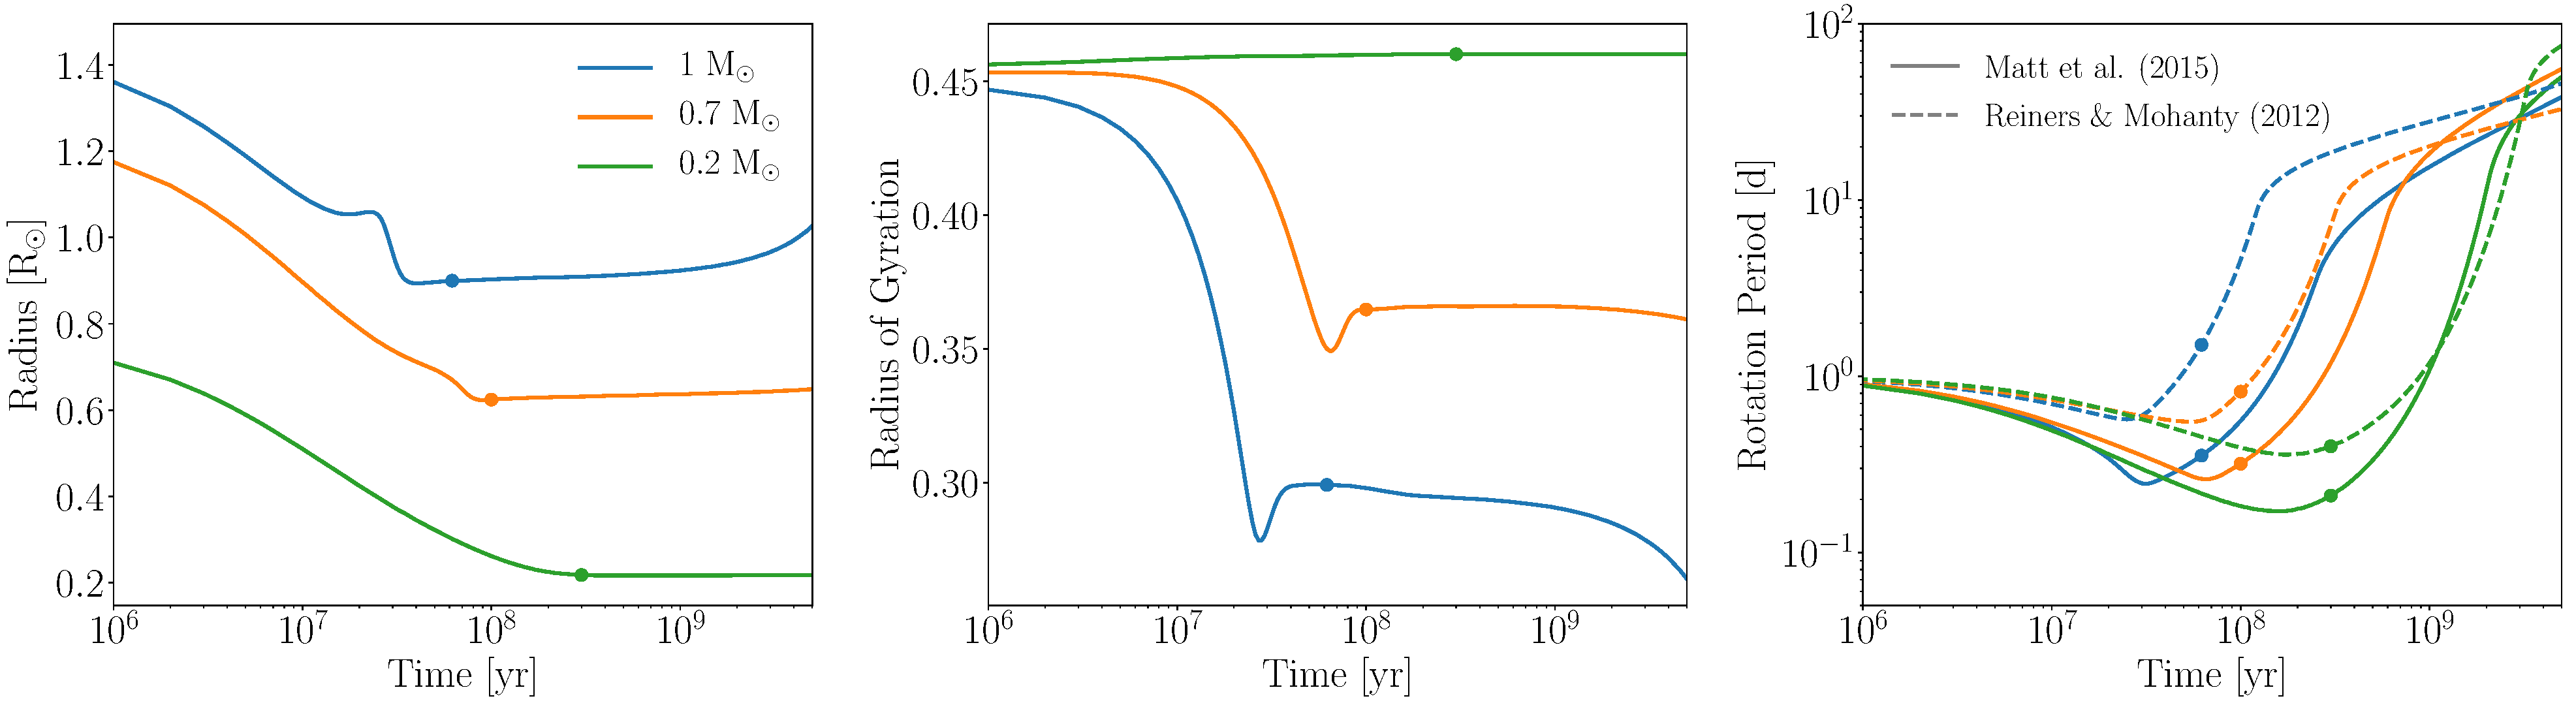
\includegraphics[width=\textwidth]{../Plots/stellarExample.pdf}
   \caption{Stellar $R$ (left), $r_g$ (middle), and P$_{rot}$ (right) evolution for 0.2 M$_{\odot}$ (M, green), 0.7 M$_{\odot}$ (K, orange), and 1 M$_{\odot}$ (G, blue) mass stars computed according to \stellar, our interpolation of the \citet{Baraffe2015} stellar evolution models ($\S$~\ref{sec:methods:stellar}) combined with the \citet{Matt2015} (solid) and \citet{Reiners2012} (dashed) magnetic braking equations. Each dot denotes the approximate time when each star reaches the main sequence.}%
    \label{fig:stellarExample}%
\end{figure*}

\subsection{Tidal Evolution} \label{sec:methods:eqtide}

 Equilibrium tidal models, first introduced by \citep{Darwin1880}, track the secular evolution of an orbiter's semi-major axis, $a$, eccentricity, $e$, and the rotation rates, $\omega$, and obliquities $\psi$, of both gravitating bodies due to tidal torques. Equilibrium tidal models assume that tidally-interacting bodies raise tidal bulges on their companions that remain offset from the line connecting the bodies' centers of mass due to friction within each body. This assumption is typically referred to as the ``weak friction approximation" \citep{Zahn2008}.  The tidal bulges cause torques that permit the exchange of angular momentum between the orbit and both bodies' spins. Equilibrium tidal models are linear since they assume that the tidal waves that comprise the tidal bulge raised on a body are uncoupled. Under these assumptions, the tidal evolution is analogous to a driven, damped harmonic oscillator \citep{Greenberg2009}. For low-mass stars, equilibrium tidal models assume that tidal forces primarily dissipate energy in the outer-convective regions via viscous turbulence \citep[see][]{Zahn2008}. Although simple, equilibrium tidal models have been used to robustly model the secular orbital and rotation evolution of both Solar System bodies and exoplanets \citep[e.g.][]{Goldreich1966,Jackson2009,Leconte2010,Heller2011,Barnes2013,Barnes2017} and stellar binaries \citep[e.g.][]{Zahn1989,Zahn2008,Khaliullin2011,Repetto2014,Fleming2018}. We refer the reader to \citet{Barnes2017} for an in-depth discussion of the assumptions and limitations of equilibrium tidal models. Here, we consider two common equilibrium tidal models to study the secular spin-orbital evolution of low-mass stellar binaries.  

\subsubsection{Constant Phase Lag Model}

The ``Constant Phase Lag" (CPL) \citep[][]{FerrazMello2008,Heller2011} equilibrium tidal model assumes that the tidal torque on one body due to its companion arises from a linear combination of several discrete, uncoupled tidal bulges, each with their own associated frequency, that maintain a fixed phase with respect to the line connecting the two stars' centers of mass. We use the \eqtide implementation of the CPL model in VPLanet following the derivation of \citet{FerrazMello2008}.  The equations that govern the secular change in $e$ and $a$ are as follows:

\begin{equation} \label{eqn:cpl:e}
\frac{de}{dt} = -\frac{ae}{8 G m_1 m_2} \sum_{i=1}^2 Z_{i,\mathrm{CPL}} \left( 2 \varepsilon_{0,i} - \frac{49}{2} \varepsilon_{1,i} + \frac{1}{2} \varepsilon_{2,i} + 3 \varepsilon_{5,i} \right)
\end{equation}
\begin{equation} \label{eqn:cpl:a}
\frac{da}{dt} = \sum_{i=1}^2 \frac{da_i}{dt}
\end{equation}
where if the $i^{th}$ body is tidally-locked in a synchronous orbit,
\begin{equation} \label{eqn:cpl:dadt_locked}
\frac{da_{i,sync}}{dt} = -\frac{a^2}{G m_1 m_2} Z_{i,\mathrm{CPL}} \left( 7 e^2 + \sin^2 (\psi_i) \right) \varepsilon_{2,i},
\end{equation}
otherwise
\begin{equation}
\begin{split}
\frac{da_i}{dt} & = \frac{a^2}{4 G m_1 m_2} Z_{i,\mathrm{CPL}} \left( 4 \varepsilon_{0,i} + e^2 \left[ -20 \varepsilon_{0,i} + \frac{147}{2} \varepsilon_{1,i} \right. \right. \\
&  + \left. \left. \frac{1}{2} \varepsilon_{2,i} - 3 \varepsilon_{5,i} \right] - 4 \sin^2 (\psi_i) \left[ \varepsilon_{0,i} - \varepsilon_{8,i} \right] \right).
\end{split}
\end{equation}
The CPL equations for $\psi$ and $\omega$ evolution are
\begin{equation} \label{eqn:cpl:psi}
\frac{d\psi_i}{dt} = \frac{Z_{i,\mathrm{CPL}} \sin(\psi_i)}{4 m_i r_{g,i}^2 R_i^2 n \omega_i} \left( [1-\xi_i] \varepsilon_{0,i} + [1+\xi_i](\varepsilon_{8,i} - \varepsilon_{9,i}) \right)
\end{equation}
\begin{equation} \label{eqn:cpl:omega}
\begin{split}
\frac{d\omega_i}{dt}& = -\frac{Z_{i,\mathrm{CPL}}}{8m_i r_{g,i}^2 R_i^2 n} \left(4 \varepsilon_{0,i} + e^2\left[-20\varepsilon_{0,i} + 49\varepsilon_{1,i} + \varepsilon_{2,i} \right] \right. \\
& \left. + 2 \sin^2(\psi_i) \left[ -2 \varepsilon_{0,i} + \varepsilon_{8,i} + \varepsilon_{9,i} \right] \right)
\end{split}
\end{equation}
where $G$ is Newton's gravitational constant, $n$ is the binary's mean motion, and the index $i$ denotes that $i^{th}$ body. The tidal phase lags signs, $\varepsilon$, for the $i^{th}$ body are given by
\begin{equation} \label{eqn:cpl:eps}
\begin{split}
\varepsilon_{0,i} & = \Sigma(2 \omega_i - 2n) \\
\varepsilon_{1,i} & = \Sigma(2 \omega_i - 3n) \\
\varepsilon_{2,i} & = \Sigma(2 \omega_i - n) \\
\varepsilon_{5,i} & = \Sigma(n) \\
\varepsilon_{8,i} & = \Sigma(\omega_i - 2n) \\
\varepsilon_{9,i} & = \Sigma(\omega_i)
\end{split}
\end{equation}
where the function $\Sigma(x)$ returns $1$ for positive $x$, $-1$ for negative $x$, and $0$ otherwise.

The intermediate variable $Z_{\mathrm{CPL},i}$ is given by
\begin{equation} \label{eqn:cpl:z}
Z_{i,\mathrm{CPL}} = 3 G^2 k_{2,i} M_j^2 (M_i + M_j) \frac{R_i^5}{a^9} \frac{1}{n Q_i}
\end{equation}
where the $j^{th}$ body is the $i^{th}$ body's companion, $k_{2}$ is the body's Love number of degree 2, and $Q$ is the tidal quality factor (``tidal Q"). The tidal Q parameterizes the energy dissipation due to tidal evolution, with lower tidal Qs, i.e. larger phase differences between the tidal bulges, driving more rapid tidal evolution.

The other intermediate variable, $\xi_i$, is defined as
\begin{equation}\label{eqn:cpl:chi}
\xi_i = \frac{r_{\mathrm{g},i}^2 R_i^2 \omega_i a n }{ G M_j}.
\end{equation}

\subsubsection{Constant Time Lag Model}

The ``Constant Time Lag" (CTL) \citep[][]{Hut1981,Leconte2010} equilibrium tidal model assumes a constant time interval between the body's tidal bulge and the passage of the tidally-interacting companion. In this formalism, unlike the CPL model, the CTL model is continuous over a range of tidal wave frequencies and applicable for large $e$.  However if the assumption of linearity is relaxed, i.e. frequencies associated with tidal bulges are allowed to depend on a spin or orbital forcing frequency, then this model is only valid over a small range of frequencies \citep{Greenberg2009}, hence we do not make this assumption and hold the tidal time lag fixed. We use the \eqtide implementation of the CTL model in VPLanet following the derivation of \citet{Leconte2010}.  The equations that govern the secular changes in $e$, $a$, $\omega$, and $\psi$ are as follows:

\begin{equation} \label{eqn:ctl:e}
  \frac{de}{dt} = \frac{11 ae}{2 G M_1 M_2}
  \sum_{i = 1}^2 Z_{\mathrm{CTL},i} \left( \cos(\psi_i) \frac{f_4(e)}{\beta^{10}(e)}  \frac{\omega_i}{n} -\frac{18}{11} \frac{f_3(e)}{\beta^{13}(e)}\right),
\end{equation}

\small
\begin{equation}\label{eqn:ctl:a}
  \frac{da}{dt} \ = \  \frac{2 a^2}{G M_1 M_2}
  \sum\limits_{i = 1}^2 Z_{\mathrm{CTL},i} \left( \cos(\psi_i) \frac{f_2(e)}{\beta^{12}(e)} \frac{\omega_i}{n} - \frac{f_1(e)}{\beta^{15}(e)}\right),
\end{equation}

\begin{equation}\label{eqn:ctl:omega}
  \frac{d\omega_i}{dt} \ = \ \frac{Z_{\mathrm{CTL},i}}{2 M_i r_{g,i}^2 
R_i^2 n} \left( 2 \cos(\psi_i) \frac{f_2(e)}{\beta^{12}(e)} - \left[ 1+\cos^2(\psi)
 \right] \frac{f_5(e)}{\beta^9(e)} 
\frac{\omega_i}{n} \right),  
\end{equation}
and
\begin{equation}\label{eqn:ctl:psi}
  \frac{d\psi_i}{dt} = \frac{Z_{\mathrm{CTL},i} \sin(\psi_i)}{2 M_i r_{g,i}^2 R_i^2 n \omega_i}\left( \left[ \cos(\psi_i) - \frac{\xi_i}{ \beta} \right] \frac{f_5(e)}{\beta^9(e)} \frac{\omega_i}{n} - 2 \frac{f_2(e)}{\beta^{12}(e)} \right).
\end{equation}
\normalsize
where the intermediate variables are given by 
\begin{equation}\label{eqn:ctl:z}
 Z_{i,\mathrm{CTL}} = 3 G^2 k_{2,i} M_j^2 (M_i+M_j) \frac{R_i^5}{a^9} \tau_i ,
\end{equation}
and 
\begin{equation}\label{eqn:ctl:f_e}
\begin{array}{l}
\beta(e) = \sqrt{1-e^2},\\
f_1(e) = 1 + \frac{31}{2} e^2 + \frac{255}{8} e^4 + \frac{185}{16} e^6 + \frac{25}{
64} e^8,\\
f_2(e) = 1 + \frac{15}{2} e^2 + \frac{45}{8} e^4 + \frac{5}{16} e^6,\\
f_3(e) = 1 + \frac{15}{4} e^2 + \frac{15}{8} e^4 + \frac{5}{64} e^6,\\
f_4(e) = 1 + \frac{3}{2} e^2 + \frac{1}{8} e^4,\\
f_5(e) = 1 + 3 e^2 + \frac{3}{8} e^4.
\end{array}
\end{equation}

In both the CPL and CTL model, We assume $k_2 = 0.5$. This choice of $k_2$ does not impact our results as $k_2$ is degenerate with Q in the CPL model, e.g. the $k_2/Q$ scaling in Eq.~(\ref{eqn:cpl:z}), and with $\tau$ in the CTL model, e.g. $k_2 \tau$ scaling in Eq.~(\ref{eqn:ctl:z}), so we instead examine how our results scale with $Q$ and $\tau$.  Any constraints we derive as a function $Q$ or $\tau$ can trivially be scaled to other values of $k_2$.

\subsubsection{Tidal Locking}

Tidal torques drive a body's rotation rate towards the tidally-locked state. When a body tidally locks, tidal torques fix P$_{rot}$ to the equilibrium P$_{rot}$, P$_{eq}$.  Typically, tidal locking is understood in the context of a synchronized rotator, e.g. when P$_{rot} = $ P$_{eq} = $ P$_{orb}$. Although spin-orbit synchronization is an expected outcome of tidal evolution \citep{Counselman1973}, in general for tidally-locked bodies on non-circular orbits, both the CPL and CTL model predict pseudosynchronous, or supersynchronous rotation, e.g. Mercury's 3:2 spin-orbit resonance \citep[P$_{rot} = 2/3$ P$_{orb}$,][]{GoldreichPeale1966}.   

The CPL model, owing to its assumption of a finite number of discrete tidal lags, only permits a 1:1 and 3:2 spin-orbit state where, following \citet{Barnes2017}, the CPL P$_{eq}$ is given by
\begin{equation} \label{eqn:cpl:eqPer}
P^{\mathrm{CPL}}_{eq} = 
\begin{cases}
P_{orb} & \text{if } e < \sqrt{1/19}\\
\frac{2}{3}P_{orb} & \text{if } e \geq \sqrt{1/19}.
\end{cases}
\end{equation}
Therefore, the CPL model predicts synchronous rotation for $e \lsim 0.23$, and a supersychronous 3:2 spin-orbit state otherwise for tidally-locked rotators.

We note that two discrete rotation states are not the only permitted ones for tidally-locked systems under the CPL formalism. For example, an alternate derivation of P$_{eq}$ for orbiters with rotation axes perpendicular to the orbital plane under the CPL model predicts
\begin{equation} \label{eqn:cpl:eqPerCont}
P_{eq} = \frac{P_{orb}}{1 + 9.5e^2},
\end{equation}
a continous function of $e$ \citep{Goldreich1966b,Murray1999}. Here, we follow the suggestions of both \citet{Barnes2013} and \citet{Barnes2017} and use the discrete P$_{eq}$ version of the CPL model for self-consistency.

The CTL model is continuous over a range of tidal frequencies and therefore predicts a P$_{eq}$ that is a continuous function of both $e$ and $\psi$.  Following \citet{Barnes2017}, we define the CTL P$_{eq}$ by
\begin{equation} \label{eqn:ctl:eqPer}
P^{\mathrm{CTL}}_{eq} = P_{orb} \frac{\beta^3 f_5(e) (1 + \cos^2(\psi))}{2f_2(e) \cos(\psi)}.
\end{equation}
The CTL model predicts that bodies on eccentric orbits tidally-lock into supersyncronous rotation, and only bodies with aligned spins on circular orbits are synchronous rotators. 

In general, a continuous P$_{eq}$ and the discrete 1:1 and 3:2 spin-orbit commensurabilities are not the only equilibrium rotation states for tidally-locked rotators predicted by equilibrium tidal models. For example, \citet{Rodriguez2012} show that tidally-interacting bodies can get captured into many spin-orbit resonances states, e.g. 2:1, 5:2, 4:3, etc. Although our models do not resolve capture into such states, we search for evidence of them in data of the spin-orbital states \kepler EBs.

\subsubsection{Numerical Details of Tidal Locking}

Due to the discontinuities in the equilibrium tidal model equations, for example in Eq.~(\ref{eqn:cpl:eps}) when $\omega \approx n$, and due to the inherant discreteness of numerical integrations, numerical solutions for the CPL and CTL models can produce unphysical evolution. We follow \citet{Barnes2013} and \citet{Fleming2018} and fix P$_{rot} = $ P$_{eq}$ according to Eq.~(\ref{eqn:cpl:eqPer}) or Eq.~(\ref{eqn:ctl:eqPer}) for the CPL and CTL models, respectively, when P$_{rot}$ is within $1\%$ of P$_{eq}$.  To ensure that tidal torques dominate over torques due to magnetic braking and stellar evolution when forcing tidal-locking, we additionally require that the P$_{rot}$ derivative points towards $P_{eq}$ on both sides of P$_{eq}$, i.e. when the gradient of P$_{rot}$ points towards the tidally-locked state, before fixing P$_{rot} = $ P$_{eq}$. We find that this scheme produces physically and numerically accurate results. 

\subsubsection{Example Tidal Evolution} \label{sec:methods:eqtideExample}

We plot the tidal evolution for $a$, $e$, and $\omega$, ignoring stellar evolution, for a solar-twin binary with an initial P$_{orb} = 10$ d, P$_{rot} = 1$ d, $e = 0.2$ for the CPL model and CTL model, assuming $Q=10^6$ and $\tau = 0.1$ seconds, respectively, in Fig.~\ref{fig:tidalExample}. Both the CPL and CTL model predict the same qualitative evolution: both the binary's $e$ and P$_{orb}$ slightly increase as tides force the spins toward the tidally-locked state, transferring rotational angular momentum into the orbit in the process.  At late times, both the CPL and CTL drive the binaries towards orbital circularization, with tidal dissipation decreasing P$_{orb}$. The predictions of the CPL and CTL model, differ, however, when the binaries tidally-lock.  Under the CPL model, the binary tidally-locks into a synchronous orbit when $e < \sqrt{1/19}$, e.g. Eq.~(\ref{eqn:cpl:eqPer}), while the CTL model predicts supersyncronous rotation due to the CTL model's equilibrium period eccentricity dependence, e.g. Eq.~(\ref{eqn:ctl:eqPer}).

\begin{figure}
	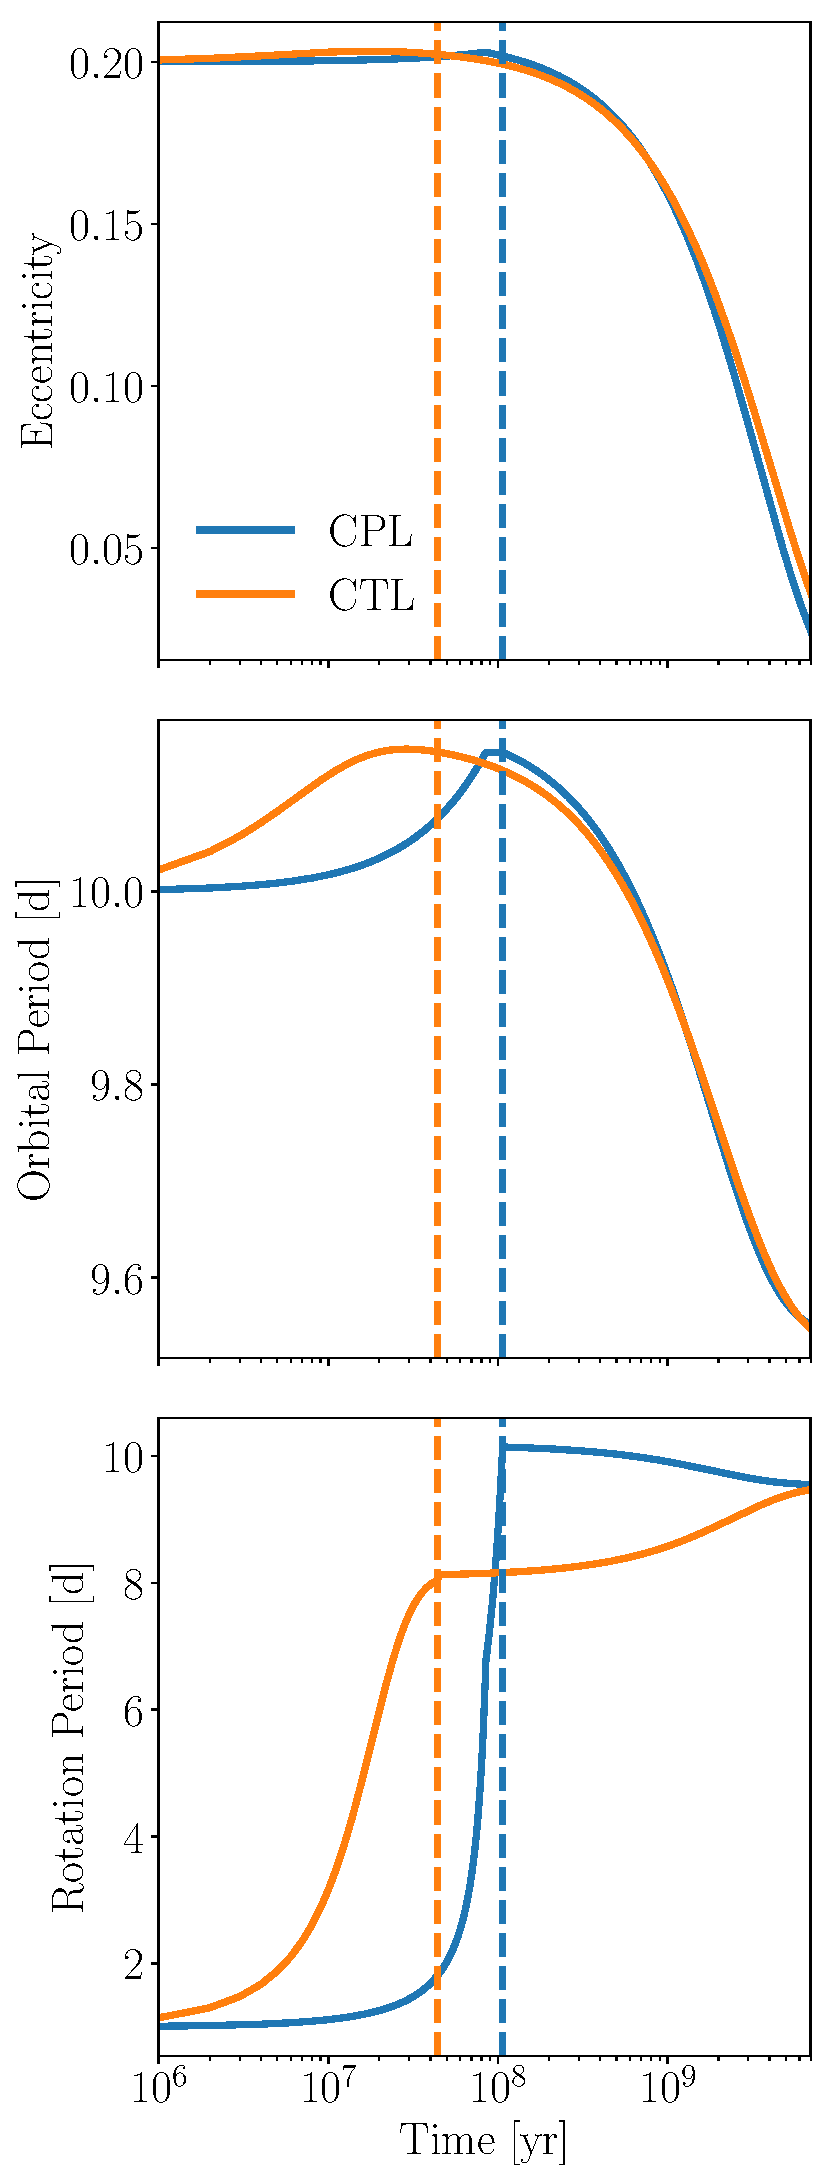
\includegraphics[width=0.4\textwidth]{../Plots/tidalExample.pdf}
   \caption{Tidal evolution of a 1 M$_{\odot} -$ 1 M$_{\odot}$ stellar binary's $e$ (top), P$_{orb}$ (middle) and P$_{rot}$ (bottom) for the CPL (blue) and CTL (orange) model. The blue (CPL) and orange (CTL) vertical dashed lines denote when the stellar binary tidally locks. Both the CPL and CTL model predict the same qualitative evolution. The rotational evolution differs, however, as under the CPL model, the binary tidally-locks into a synchronous orbit as $e < \sqrt{1/19}$, e.g. Eq.~(\ref{eqn:cpl:eqPer}), while the CTL model predicts supersyncronous rotation due to the CTL model's equilibrium period eccentricity dependence (see Eq.~(\ref{eqn:ctl:eqPer})).}%
    \label{fig:tidalExample}%
\end{figure}

\subsection{Coupled Stellar-Tidal Evolution For Tidally-Locked Systems} \label{sec:coupled}

Following \citet{Fleming2018}, when one or both binary stars are tidally locked, tidal forces prevent magnetic braking from spinning down the tidally-locked star(s), and any angular momentum lost comes at the expense of the binary orbit, decreasing $a$ as a result \citep{Verbunt1981}.  Below in Eq.~(\ref{eqn:tidal_locked_one}) and Eq.~(\ref{eqn:tidal_locked_two}), we modify the $a$ decay equations due to stellar evolution and magnetic braking in tidally-locked binaries from \citet{Fleming2018}, their Eqs. (18) and (20), to additionally account for $r_g$ evolution when one or both stars tidally-lock, respectively, assuming conservation of angular momentum:
\small
\begin{equation} \label{eqn:tidal_locked_one}
\begin{split}
\dot{a}_{coupled}^{(1)} = \frac{-\dot{J}_{mb} - 2 \omega \left( m_1 r_{g,1}^2 R_1 \dot{R_1} - m_1 r_{g,1} \dot{r}_{g,1} R_1^2 \right)}
{\frac{\mu^2 G M (1-e^2)}{2J_{orb}} - \frac{3 \omega}{2a} m_1 r_{g,1}^2 R_1^2}
\end{split}
\end{equation}
\normalsize
and
\small
\begin{equation} \label{eqn:tidal_locked_two}
\begin{split}
\dot{a}_{coupled}^{(2)} = \frac{-\dot{J}_{mb} - 2 \omega \left( \sum_{i=1}^{2} m_i r_{g,i}^2 R_i \dot{R_i} + m_i r_{g,i} \dot{r}_{g,i} R_i^2 \right)}
{\frac{\mu^2 G M (1-e^2)}{2J_{orb}} - \frac{3 \omega}{2a} \left( m_1 r_{g,1}^2 R_1^2 + m_2 r_{g,2}^2 R_2^2 \right)}
\end{split}
\end{equation}
\normalsize
where $J_{orb}$ is the orbital angular momentum.

%% SECTION: Simulations + Initial conditions %%
\section{Simulations} \label{sec:simulations}

We examine stellar angular momentum evolution in low-mass binaries by simulating four sets of 10,000 stellar binaries, one modeled using the CPL model and the other using the CTL formalism, using both magnetic braking models.  We simulate both stars' spin evolution but mainly consider the P$_{rot}$ evolution for the primary, i.e. more massive star in binaries, as it is observationally easier to measure a P$_{rot}$ on the more massive, and hence brighter, star \citep[e.g.][]{Meibom2006,Lurie2017}. For each simulation, we sample the primary's mass uniformly over $[0.1, 1]$ M$_{\odot}$. Following \citet{Matt2015}, we uniformly sample the log$_{10}$ of P$_{rot}$ over [$0.8,15$] days, a distribution that approximates the P$_{rot}$ distribution of young stars in the ${\sim}2$ Myr old Orion Nebula Cluster \citep{Stassun1999,Herbst2001,Herbst2002,Rodriguez-Ledesma2009}.  We compute the secondary star's mass by uniformly sampling the mass ratio over [$0.1, 1$] following observations of mass ratios in low-mass binaries \citep{Raghavan2010,Moe2018}. Given the inherent uncertainty in and complexity of the formation of short-period binaries \citep[e.g.][]{Bonnell1994,Bate2000,Bate2002,Moe2018} and the potential for dynamical processing via tides or stellar close encounters \citep[e.g.][]{Mardling2001,Hurley2002,Ivanova2005,Meibom2005}, we take an agnostic approach to the initial orbital configuration by uniformly randomly sampling the initial eccentricity ($e$) over [$0.0,0.3$], consistent with eccentricities of field binaries that likely have not been tidally-processed \citep{Raghavan2010}. Although the CTL model is applicable for $e \gsim 0.3$, the CPL model is not, so we restrict $e \leq 0.3$ to allow us to compare both models.
We uniformly sample the initial P$_{orb}$ over [$3,100$] d and do not consider P$_{orb} < 3$ d as these binaries are likely to have a tertiary companion \citep{Tokovinin2006} which can significantly impact the inner binary's dynamical evolution \citep[e.g.][]{Munoz2015,Martin2015b,Hamers2016,Moe2018}. 

Values for stellar tidal $Q$s and $\tau$s for low-mass stars are highly uncertain due to complex viscous evolution within the stars \citep{Ogilvie2007}, and can differ for stars of the same spectral class \citep{Barker2009}. These parameters can also vary as a function of stellar mass or age \citep{Bolmont2016,vanEylen2016}, likely due to low-mass stars' evolving convective regions where the tidal dissipation predominantly occurs \citep{Zahn2008}. Typical values of $Q$ and $\tau$ for Sun-like stars are estimated to be of order $Q \approx 10^6$ and $\tau \approx 0.1$ s, respectfully \citep[e.g.][]{Meibom2005,Ogilvie2007,Jackson2008}, however a range of values exist in the literature.  Therefore, we consider a wide range of tidal parameters by sampling stellar tidal $Q$s log-uniformly over $[10^4,10^8]$ and $\tau$ log-uniformly over $[10^{-2},10]$ s.  There is no general expression to compute $Q$ as a function of $\tau$, or vice versa, except in some special cases where approximations exist, e.g. Eqn. (2) from \citet{Heller2011}. 

We explore the impact of both the \citet{Matt2015} and \citet{Reiners2012} magnetic braking models, but default to using the \citet{Matt2015} unless noted otherwise. All stars have an initial age of 5 Myr unless stated otherwise as by this time, the gaseous protoplanterary circumbinary disk that can drive significant dynamical evolution in the binary \citep[e.g.][]{Fleming2017} would likely have dissipated \citep{Haisch2001}.

We also perform a smaller subset of simulations to illustrate the behaviour of our coupled model and describe their initial conditions as we introduce them. All code used to run simulations and generate figures is available online\footnote{\href{https://github.com/dflemin3/sync}{https://github.com/dflemin3/sync}.} with accompanying descriptions and documentation.

%% SECTION: RESULTS %%

\section{Results} \label{sec:results}

\subsection{Interaction Between Magnetic and Tidal Braking} \label{sec:eq}

Here we examine the P$_{rot}$ evolution of 1 M$_{\odot} - 1$ M$_{\odot}$ binaries on initially circular orbits with a focus on systems with weak tidal torques, i.e. long P$_{orb}$ and large $Q$ or small $\tau$, to identify the boundary between evolution dominated by tides or magnetic braking.  

\subsubsection{Analytic Torque Balance}

In the weak tides regime, spin-down due to magnetic braking will drive the stellar P$_{rot}$ past P$_{eq}$, resulting in subsynchronous rotation. Since magnetic braking scales as P$_{rot}^{-3}$ for unsaturated rotators, e.g. Eqn.~(\ref{eqn:mattUnSat}), magnetic braking torques weaken as stellar rotation slows, so at some P$_{rot}$, tidal torques that try to spin-up sunsynchronous rotators back towards P$_{eq}$ will balance the spin-down torque of magnetic braking, producing a long-lasting state of subsynchronous rotation. Given an initial binary system configuration, we can analytically determine at which P$_{rot}$ torques due to magnetic braking and tides balance. 

We derive where this balance occurs by considering tidal torques under the CTL formalism and magnetic braking under the \citet{Matt2015} model to match the simulations performed in $\S$~\ref{sec:mattBalance}. We assume torque balance by setting the sum of Eqn.~(\ref{eqn:ctl:omega}), noting that $d\omega/dt = 1/I dJ\dt$, and Eqn.~(\ref{eqn:mattUnSat}) equal to 0. We use the unsaturated \citet{Matt2015} magnetic braking torque since in the weak tides regime, the tidal and magnetic braking torques will only balance for slow rotators, placing the stars in the unsatured regime \citep{Matt2015}. For simplicity, we assume both stars are solar-mass with 0 obliquity, the binary orbit is circular, and that the torque balance occurs on the main sequence, allowing us to set the $R = 1 R_{\odot}$. Under these assumptions, by specifying a P$_{orb}$ and $k_2 \tau$, we can compute the P$_{rot}$ at which tidal and magnetic braking torques balance.

\subsubsection{Using the \citet{Matt2015} Magnetic Braking Model} \label{sec:mattBalance}

In Fig.~\ref{fig:eqPer}, we plot the evolution of P$_{rot}$, normalized by P$_{eq}$, and its time derivative for P$_{orb} \in [5,60]$ d modeled using both the CPL (solid line, $Q=10^6$) and CTL (dashed line, $\tau = 0.1$ s) formalisms. Both models predict that binaries with P$_{orb} < 10$ d will tidally-lock within 100 Myr, in agreement with observations \citep{Meibom2005} and previous theoretical work \citep{Zahn1989}. The CPL model predicts that each binary tidally-locks, even out to P$_{orb} = 60$ d, indicating that tidal locking is not necessarily restricted to short P$_{orb}$ systems. 

\begin{figure*}
	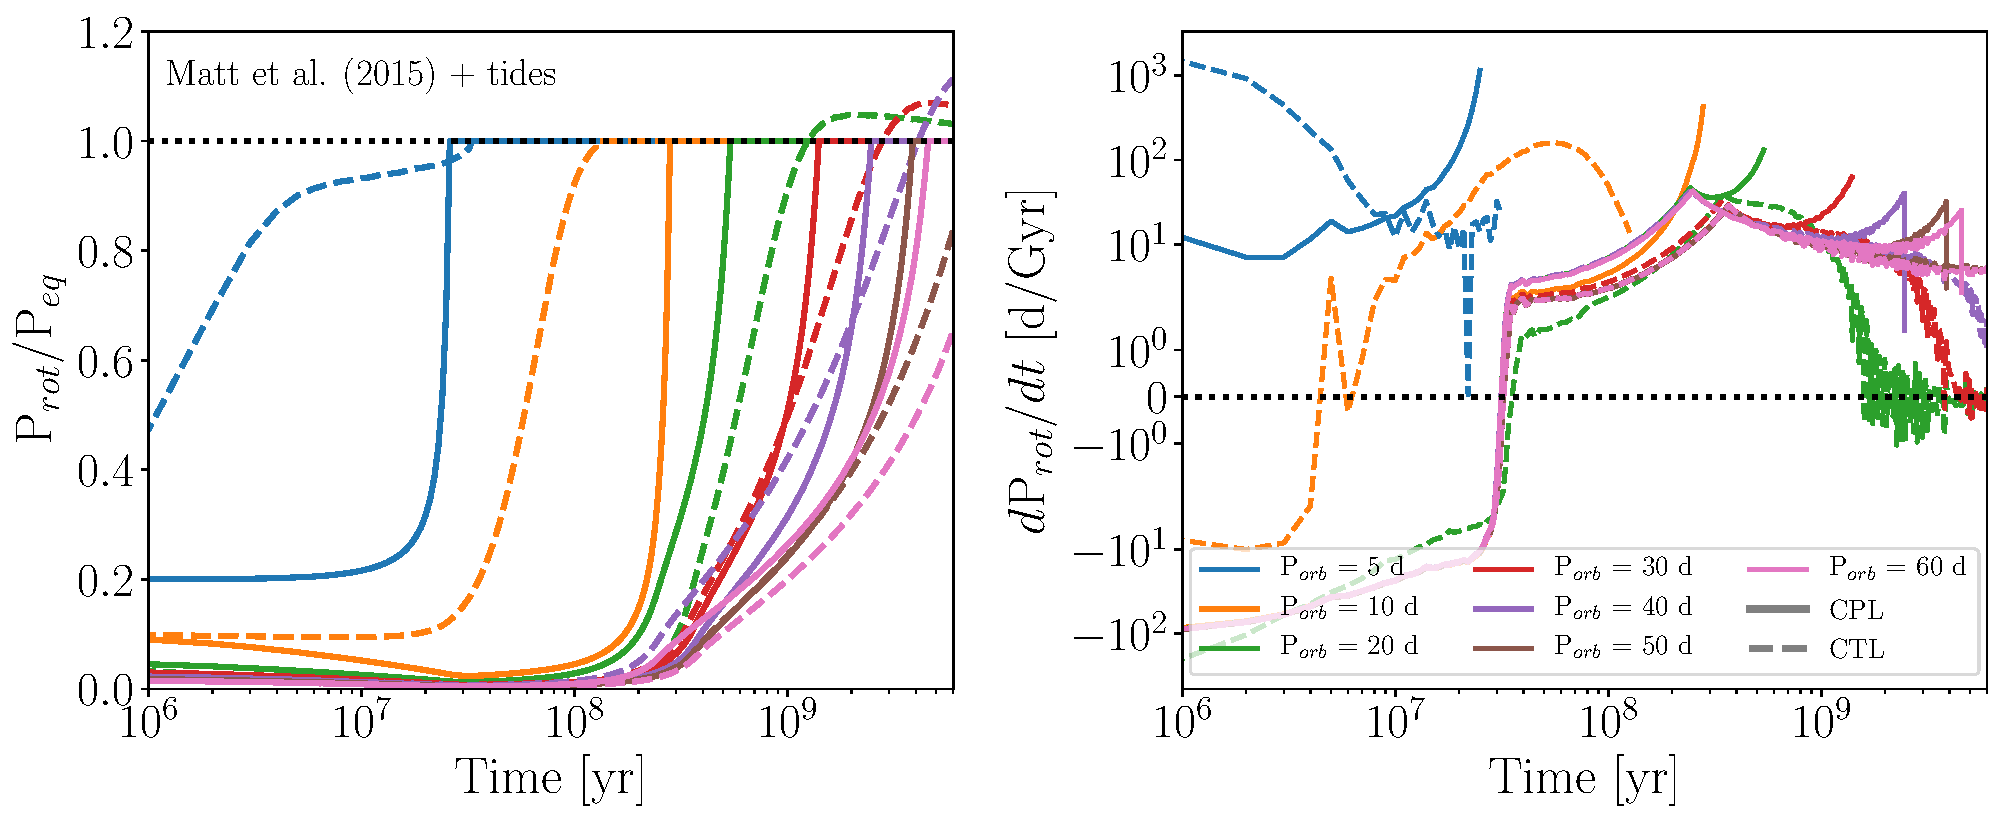
\includegraphics[width=\textwidth]{../Plots/eqPerTwoPanelMatt.pdf}
   \caption{Evolution of stellar P$_{rot}$, normalized by P$_{eq}$ (see Eqn.~(\ref{eqn:cpl:eqPer}) and Eqn.~(\ref{eqn:ctl:eqPer}), for initial circular binary orbits according to the CPL (solid) and CTL (dashed) models with $Q = 10^6$ and $\tau = 0.1$ s, respectively, using the \citet{Matt2015} magnetic braking model. Left: P$_{rot}/$P$_{eq}$ for stars with P$_{orb}$ ranging from 5 d to 60 d. The black dotted line indicates the tidally-locked state where P$_{rot} = $ P$_{eq}$.  Right: Net P$_{rot}$ derivative due to stellar evolution, tidal torques, and magnetic braking.  We truncate each curve when the binary tidally locks. For P$_{orb} \leq 10$ d, both the CPL and CTL models predict that the binaries lock into synchronous rotation.  For all P$_{orb}$, the CPL models tidally-lock into synchronous rotation whereas the CTL model predicts subsynchronous (P$_{rot} > $ P$_{eq}$) rotation that persists for Gyrs.}%
    \label{fig:eqPer}%
\end{figure*}

% caption extra: 
%In the CTL cases, magnetic braking overpowers tidal torques, spinning down the stars, preventing tidal-locking.  Tidal torques eventually overpower magnetic braking for long P$_{rot}$ \citep{Kawaler1988,Matt2015}, slowly driving the stellar rotation back towards the tidally-locked state. 
% Initially, all systems spin-up due to stellar radius contraction. Once the stars reach the main sequence at ${\sim} 60$ Myr, tidal torques and magnetic braking combine to spin down the stars towards the tidally-locked state. For many CTL models, $\dot{\mathrm{P}}_{rot} > 0$ as magnetic braking overpowers tidal torques causing sustained subsynchronous rotation.  After spinning down to long P$_{rot}$, magnetic braking weakens, allowing tidal torques to sheppard P$_{rot}$ towards P$_{eq}$ as the P$_{rot}$ derivatives stay near 0, but with a slight negative value.

The CTL model, however, predicts that for P$_{orb} \gsim 10$ d, magnetic braking overpowers weak tidal torques, spinning down the stars past the tidally-locked state. Magnetic braking pushes P$_{rot}/$P$_{eq} > 1$ with the maximum value set by the torque balance between tidal torques and magnetic braking. The maximum values grows for longer P$_{orb}$ since tides weaken with increasing binary separation, e.g. Eqn.~(\ref{eqn:ctl:z}), allowing magnetic braking to dominate the spin evolution. 

P$_{rot}$ eventually decreases back towards the tidally-locked state in the long-term due to a combination of three simultaneous physical effects.  First, as P$_{rot}$ continue to increase due to magnetic braking, magnetic braking itself weakens as its torque scales as $\omega$ or $\omega^3$ \citep{Kawaler1988}, depending on if the stars are in the saturated or unsaturated regime, respectively \citep{Matt2015}.  Second, as P$_{rot}$ increases further from the tidally-locked state, tidal torques strengthen as they try to force P$_{rot}$ back towards P$_{eq}$ (see Eqn.~(\ref{eqn:ctl:omega}), for example). Third, when P$_{rot} > $ P$_{eq}$, tides transfer angular momentum from the orbit into stellar rotations, decreasing P$_{orb}$ and strengthening tidal torques that strongly depend on the binary separation as $a^{-6.5}$.  These effects combine to shift the balance of power from magnetic braking-controlled stellar spin down to tidal torques spinning-up stars, shepherding them towards P$_{eq}$ in the long term. 

We can see this process unfold in the right panel of Fig.~\ref{fig:eqPer} where we plot the total P$_{rot}$ time derivative due to stellar evolution, magnetic braking, and tidal torques. Early on, $\dot{\mathrm{P}}_{rot} < 0$ as stars contract along the pre-main sequence until about 60 Myr when the stars reach the main sequence. After $R$ contraction, $\dot{\mathrm{P}}_{rot} > 0$ as tides and magnetic braking combine to spin down stars towards the tidally-locked state. For the CTL models with P$_{orb} > 10$ d, $\dot{\mathrm{P}}_{rot} > 0$, but $\ddot{\mathrm{P}}_{rot} < 0$ as the three processes described above gradually strengthen tidal torques relative to magnetic braking.  In the long-run, tidal torques overpower magnetic braking, with a slightly negative P$_{rot}$ derivative, slowly driving P$_{rot}$ towards P$_{eq}$ (see the P$_{orb} = 20, 40$ d cases in Fig.~\ref{fig:eqPer}). This slowly shifting torque balance produces a population of subsynchronous rotators with P$_{rot} > $ P$_{eq}$ that can persist for Gyrs.  

\subsubsection{Using the \citet{Reiners2012} Magnetic Braking Model}

The mechanism for producing subsynchronous rotation is not limited to the \citet{Matt2015} magnetic braking model, but rather is a generic outcome of the coupling of magnetic braking and weak tidal torques. The CTL model can only tidally-lock the P$_{orb} = 5$ d binary as the stronger magnetic braking under the \citet{Reiners2012} model forces the longer P$_{orb}$ binaries into subsynchronous rotation. Curiously, all CTL subsynchronous rotators seem to converge to P$_{rot}/$P$_{eq} \approx 1.1$.  In this state, tidal torques nearly balance magnetic braking, producing a long-lasting population of subsynchronous rotators, similar to what was observed above.  In the right panel of Fig.~\ref{fig:eqPerReiners}, we see that the net P$_{rot}$ derivatives for these binaries oscillate about 0, but are slightly negative due to the 3 simultaneous physical effects described above. This slight negative derivative is effectively negligible, however, as the torque balance will likely hold the binaries in subsynchronous rotation for 10s of Gyrs.  We note that in other exploratory simulations with larger $\tau$, we find that the tides do in fact eventually win out over magnetic braking in the long-run, driving P$_{rot}$ back towards P$_{eq}$.

\begin{figure*}
	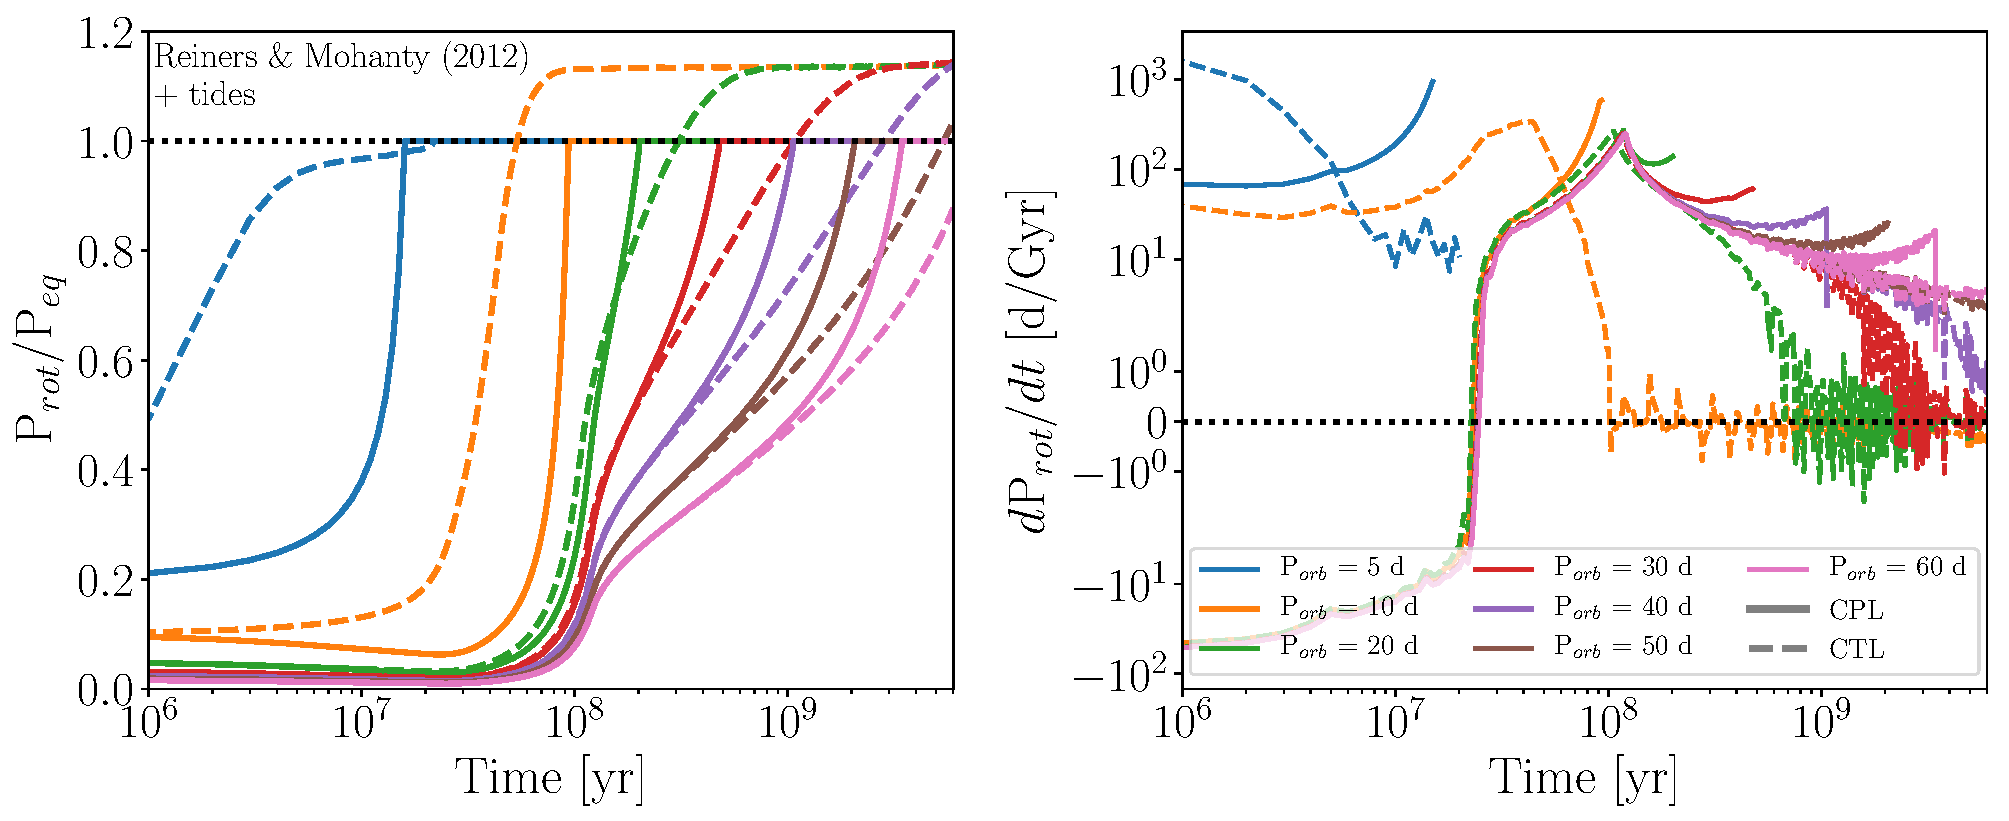
\includegraphics[width=\textwidth]{../Plots/eqPerTwoPanelReiners.pdf}
   \caption{Same format as Fig.~\ref{fig:eqPer}, but evolved using the \citet{Reiners2012} magnetic braking model.}%
    \label{fig:eqPerReiners}%
\end{figure*}

\subsubsection{Subsynchronous Rotation at Short P$_{orb}$}

In Fig.~\ref{fig:eqPerShortPorb}, we examine subsynchronous rotation in short P$_{orb}$ binaries by displaying the P$_{rot}$ evolution for a P$_{orb} = 5$ d binary for various tidal dissipation parameters. Subsynchronous rotation occurs in general for weak tidal torques, $Q>10^7$ or $\tau < 0.1$ s in these cases, and is not restricted to long P$_{orb}$ binaries. Previous theoretical studies have also predicted subsynchronous rotation in short P$_{orb}$ binaries arising from the balance between tidal torques and magnetic braking \citep[e.g.][]{Habets1989,Zahn1994,Keppens1997} suggesting that this behavior is not an artifact of our choice of tidal or magnetic braking models, but rather a general outcome of the competition between magnetic braking and tidal evolution in low-mass binaries.  Short P$_{orb}$ subsynchronous rotators can eventually tidally-lock via the mechanism described above where tidal torques gradually strengthen relative to magnetic braking. 

\begin{figure}
	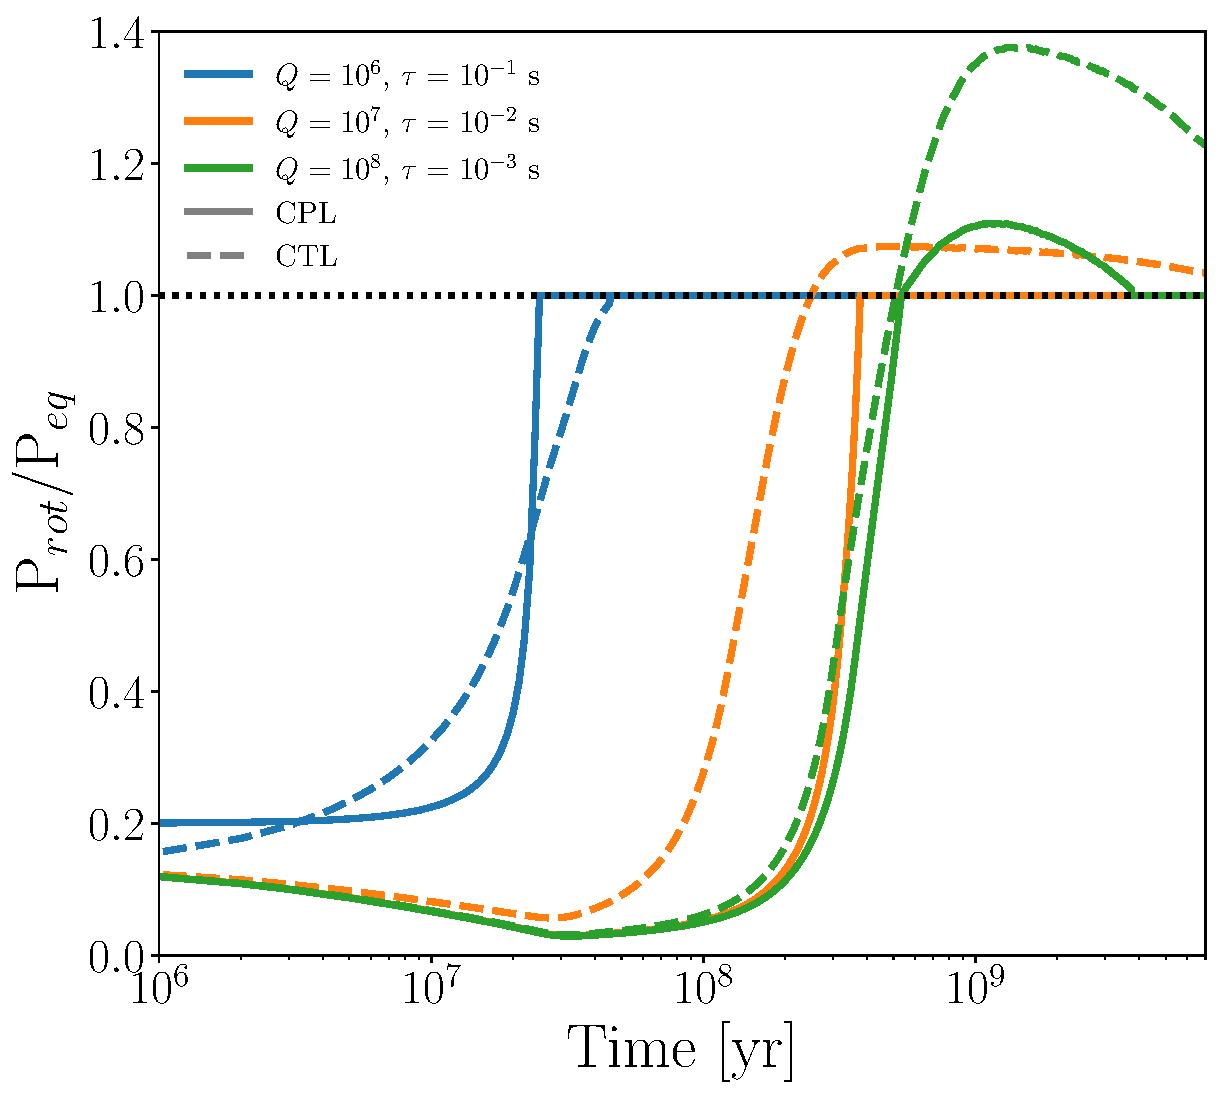
\includegraphics[width=0.45\textwidth]{../Plots/eqPerShortPorbMatt.pdf}
   \caption{Evolution of stellar P$_{rot}$, normalized by P$_{eq}$ (see Eqn.~(\ref{eqn:cpl:eqPer}) and Eqn.~(\ref{eqn:ctl:eqPer}), for initial circular binary orbits with initial P$_{orb} = 5$ d according to the CPL (solid) and CTL (dashed) models for several values of $Q$ and $\tau$, respectively, using the \citet{Matt2015} magnetic braking model. Systems with strong tidal torques ($Q = 10^6$ or $\tau = 0.1$ s) tidally lock, whereas in systems with weaker tidal torques (larger $Q$ and smaller $\tau$, respectively), magnetic braking initially overpowers tidal torques, spinning down the stars past the tidally-locked state, resulting in subsynchronous rotation. }%
    \label{fig:eqPerShortPorb}%
\end{figure}

% caption extra:
% In the long-term, magnetic braking weakens relative to tidal torques for longer P$_{rot}$, allowing tides to drive the stars back towards the tidally-locked state.

Short P$_{orb}$ subsynchronous binaries exist in nature, such as many \kepler EBs (\citet{Lurie2017}, see $\S$~\ref{sec:kepler} for further discussion), Kepler-47 \citep{Orosz2012}, EPIC 219394517 \citep{Torres2018}, and in ``Binary 6211" observed by \citet{Meibom2006}, suggesting that this theoretical observation is real and borne out in nature. Spin-orbit synchronization should therefore not be assumed for short P$_{orb}$ binaries.  We explore this effect further and test it against observations of \kepler EBs in $\S$~\ref{sec:subsync}.

\subsection{Influence of P$_{orb}$, $Q$ and $\tau$} \label{sec:qTauMaps}

We examine how P$_{rot}$ evolution in stellar binaries depends on P$_{orb}$ and the strength of tidal dissipation, parameterized by $Q$ and $\tau$ for the CPL and CTL models, respectfully. In Fig.~\ref{fig:qTauLock}, we bin our simulation results after the full 7 Gyr evolution by P$_{orb}$ and $Q$ or $\tau$ and compute the median P$_{orb}/$P$_{rot}$ in each bin, marginalizing over all other parameters.

Spin-orbit synchronization is the typical outcome for binaries with P$_{orb} < 10$ d according to the CPL model for most values of $Q$. The strong tidal torques predicted by the CPL model can even tidally-lock binaries out to P$_{orb} \approx 100 $ d for $Q < 10^5$, well beyond the expected limit of 20 d \citep{Meibom2006}.  According to the CTL model, binaries with P$_{orb} < 10$ d typically tidally-lock for $\tau \gsim 0.1$ s, and seldomly tidally-lock for P$_{orb} > 20$ d, except for systems with strong tides, $\tau \gsim 3$ s.  Both models predict a substantial population of subsynchronous rotators (red regions in Fig.~\ref{fig:qTauLock}, P$_{rot} >$ P$_{orb}$), consistent with magnetic braking dominating weak tidal torques, i.e. stars with large $Q$ or small $\tau$, that form via the mechanism described in $\S$~\ref{sec:eq}, with weaker tidal torques allowing more subsynchronous rotation.  The population of supersynchronous rotators (blue regions in Fig.~\ref{fig:qTauLock}, P$_{rot} <$ P$_{orb}$) with P$_{orb} > 80$ d does not in general correspond to binaries tidally-locking into supersynchronous rotation, but rather, typically arises from the combination of weak tidal torques and magnetic braking not spinning down stars enough for P$_{rot}$ to be close to the tidally-locked state.  

Both tidal models predict a population of nearly synchronous rotators near P$_{orb} \approx 60$ d.  This population corresponds to the evolution described in $\S$~\ref{sec:eq} in which magnetic braking initially spins down stars past the tidally-locked state, but in the long-term, tidal torques spin up the stars, shepherding them towards the tidally-locked state.  This process can keep stellar P$_{rot} \gsim$ P$_{eq}$ for several Gyrs or longer, depending on the P$_{orb}$ and $Q$ or $\tau$ (see Figs.~\ref{fig:eqPer},\ref{fig:eqPerShortPorb}). 

\begin{figure*}[ht]
	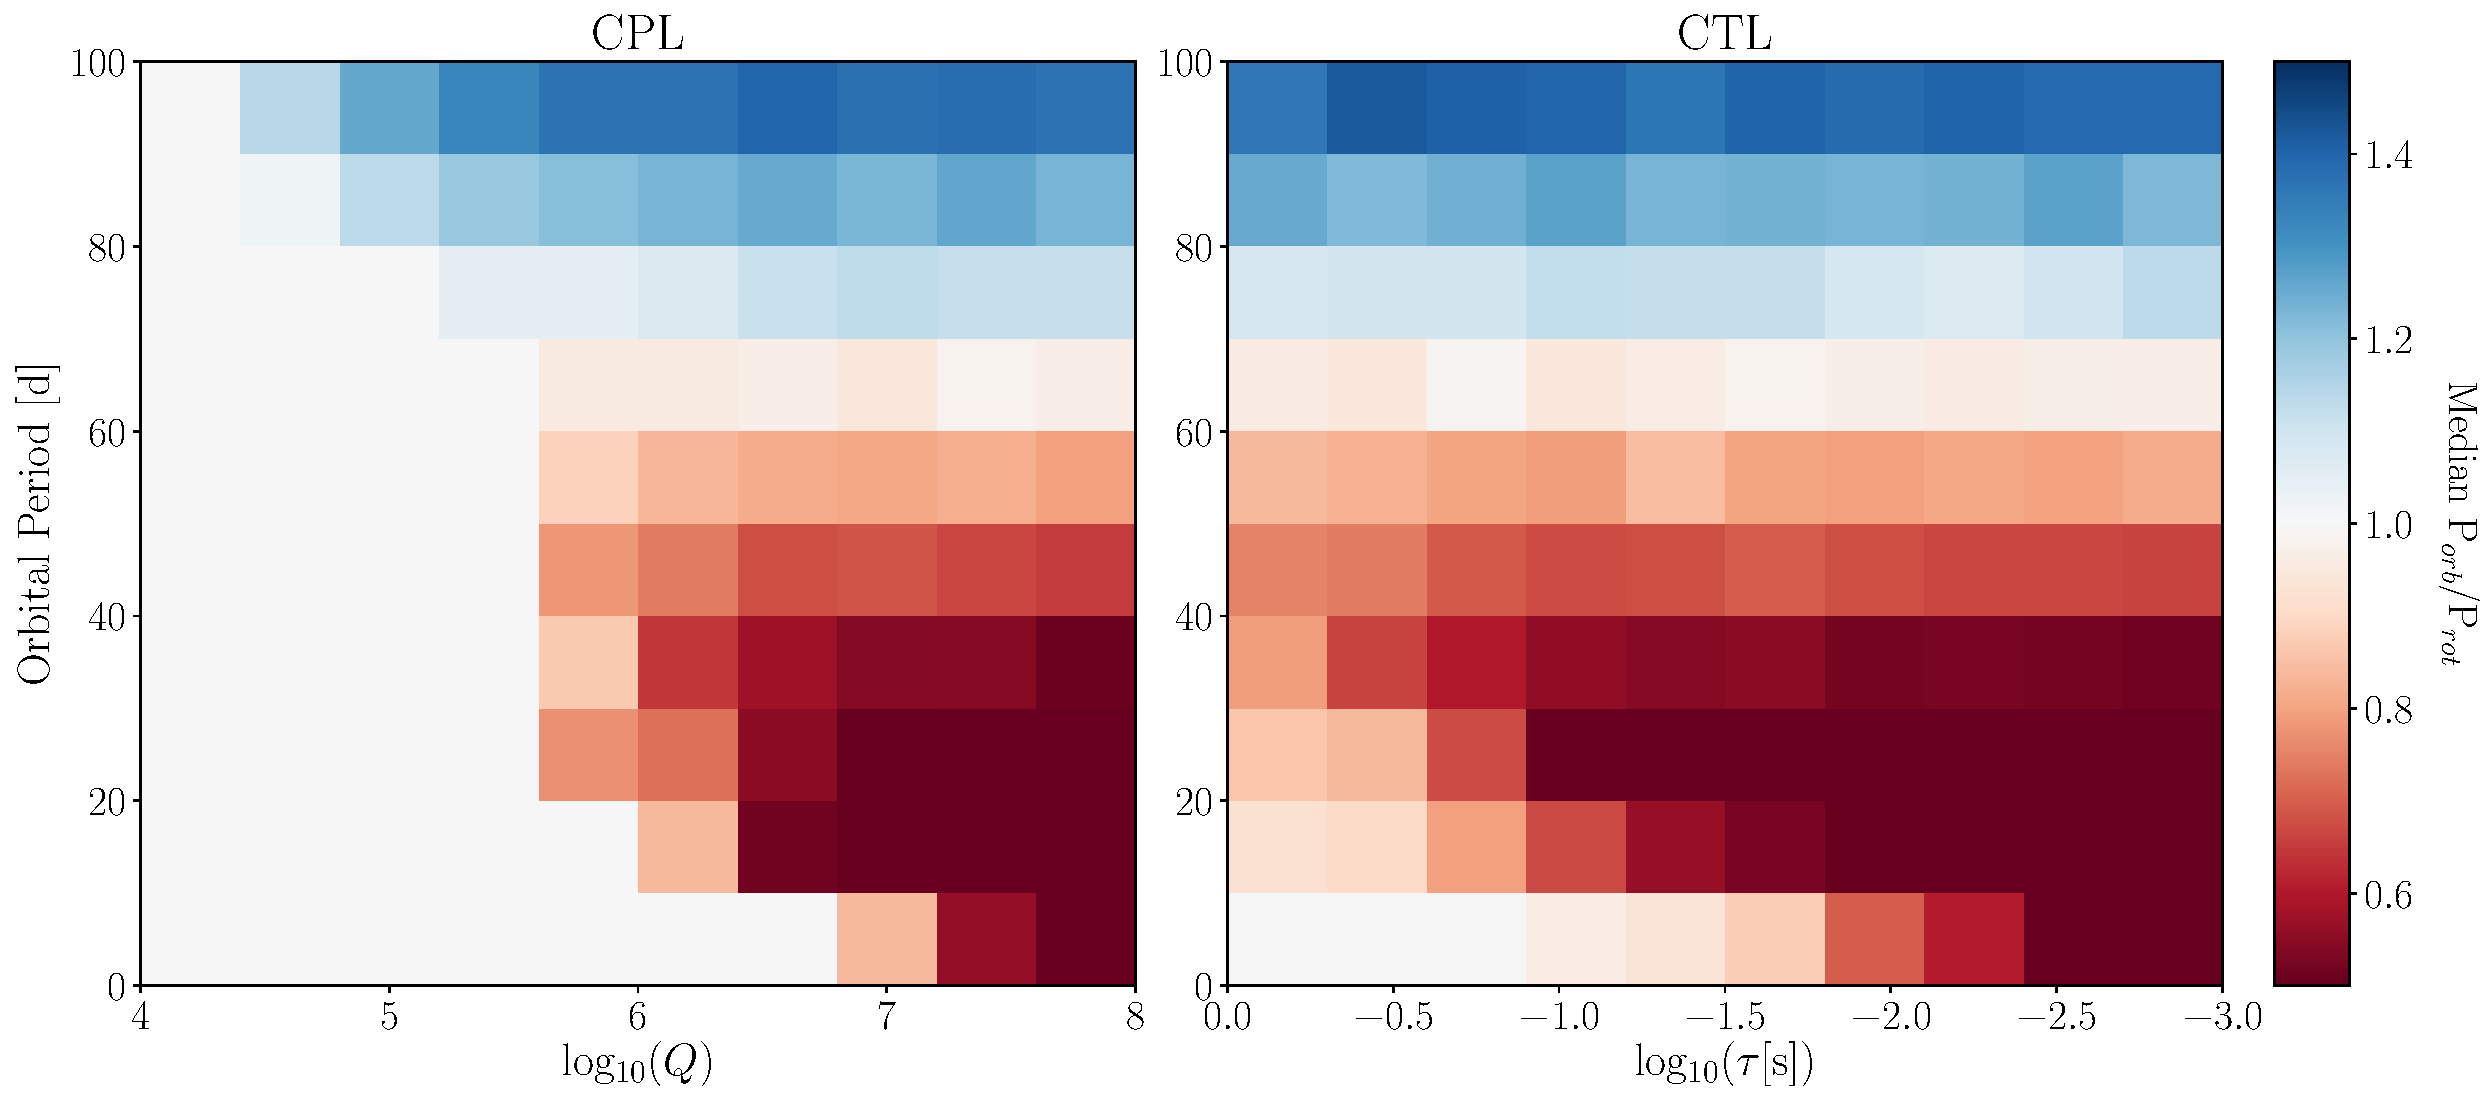
\includegraphics[width=\textwidth]{../Plots/qTauPorbRatioHist.pdf}
   \caption{Median P$_{orb}/$P$_{rot}$ at the end of the simulation according to the CPL (left) and CTL (right) models binned by log$_{10}(Q)$ and log$_{10}(\tau)$, respectively, and P$_{orb}$.  For P$_{orb} < 10$ d, the CPL model predicts that most systems will tidally lock into synchronous rotation, regardless of $Q$, whereas the CTL model requires $\tau \geq 0.1$ s to tidally-lock.  Both models exhibit supersynchronous rotation (blue regions, P$_{rot} <$ P$_{orb}$) for P$_{orb} > 80$d, that do not in general reflect tidally-locking into a supersynchronous rotation, but rather at long P$_{orb}$, the combination of weak tidal torques and magnetic braking have not spun down the star enough for P$_{rot}$ to be close to P$_{orb}$ after 7 Gyr of evolution. For large $Q$ ($> 10^{6.5}$) and small $\tau$ ($\tau < 0.1$ s), weak tidal torques cannot prevent magnetic braking from spinning down stars past the tidally-locked state, producing a population of subsynchronous rotators (red regions, P$_{rot} >$ P$_{orb}$).}%
    \label{fig:qTauLock}%
\end{figure*}

% caption extra:
% The CPL model predicts that stellar binaries can tidally-lock out to P$_{orb} = 30$ d for most values of $Q$, with some locking all the way up to P$_{orb} = 100$ d for small $Q < 10^5$.  

We isolate the impact of $Q$ and $\tau$ by binning our simulation results after 7 Gyr of evolution by P$_{orb}$ and P$_{orb}/$P$_{rot}$.  In each bin, we compute the median $Q$ and $\tau$, and the $16\%$, and $84\%$ percentiles to quantify the distribution of tidal strength parameters that are consistent with each spin-orbital state.  

\begin{figure}
	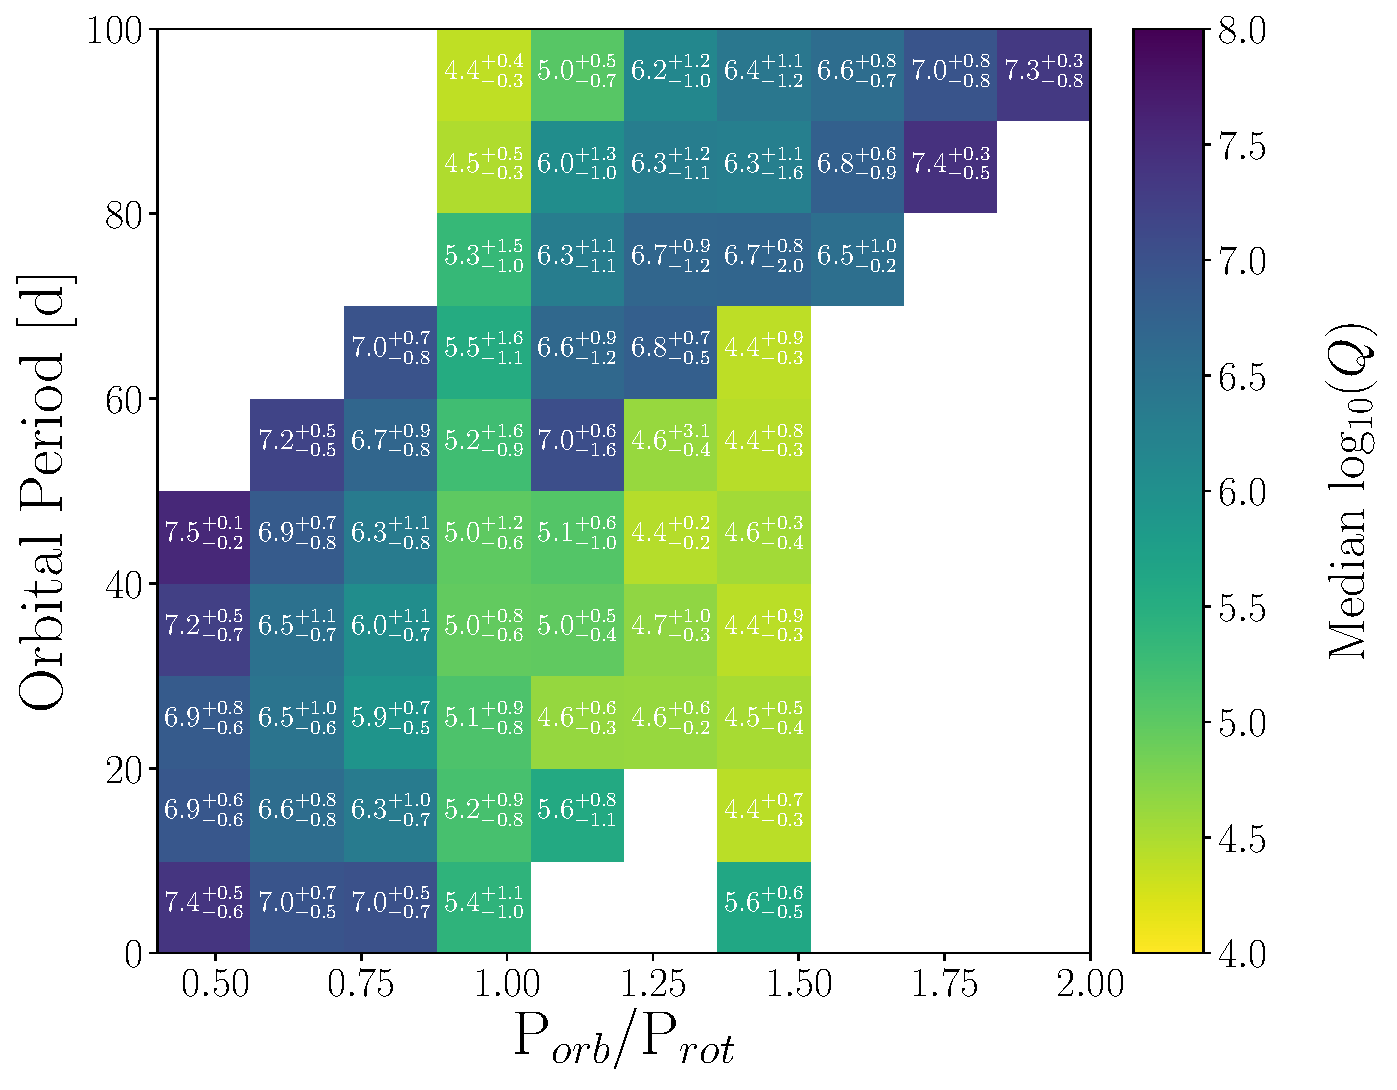
\includegraphics[width=0.45\textwidth]{../Plots/porbProtPorbQHist.pdf}
   \caption{Median log$_{10}(Q)$ of primary stars binned by P$_{orb}$ and P$_{orb}/$P$_{rot}$ evolved using the CPL model.  In each bin, we compute the median, $16\%$, and $84\%$ percentiles for log$_{10}(Q)$ and display these values. Narrow constraints imply that certain tidal parameters are required to produce that rotation state, e.g. supersynchronous rotators near P$_{orb}/$P$_{rot} = 1.5$ require $Q \lsim 10^{5.5}$. }%
    \label{fig:qmap}%
\end{figure}

For all P$_{orb}$ in Fig.~\ref{fig:qmap}, synchronous and supersynchronous rotators have systematically low $Q$s, typically $Q < 10^6$, as strong tidal torques are required to tidally-lock the systems, especially for P$_{orb} > 20$ d. For P$_{orb} < 10$ d, there are no rotators with $1.0 <$ P$_{orb}/$P$_{rot} < 1.5$ nor do any stars have P$_{orb}/$P$_{rot} > 1.5$ for P$_{orb} < 70$ d as in the CPL model, binaries with eccentric orbits can only tidally-lock into a 1:1 or 3:2 spin-orbit commensurability, i.e. Eqn.~(\ref{eqn:cpl:eqPer}).   

Subsynchronous rotators have systematically larger $Q$s, typically $Q > 10^6$, and hence experience weak tidal torques that are dominated by magnetic braking that spin-down the stars past the tidally-locked state.  This effect can be seen for P$_{orb} < 50$ d where the median $Q$ gradually increases with decreasing P$_{orb}/$P$_{rot}$, except near the tidally-locked state.  This trend reverses at longer P$_{orb} > 60$ d where supersynchronous rotation arises from the inability of tidal torques and magnetic braking to spin-down stars enough to approach the tidally-locked state by the end of the simulation.  In this case, the more supersynchronous the rotation, the weaker the tidal torques must be, and hence the larger the $Q$ must be. 

\begin{figure}
	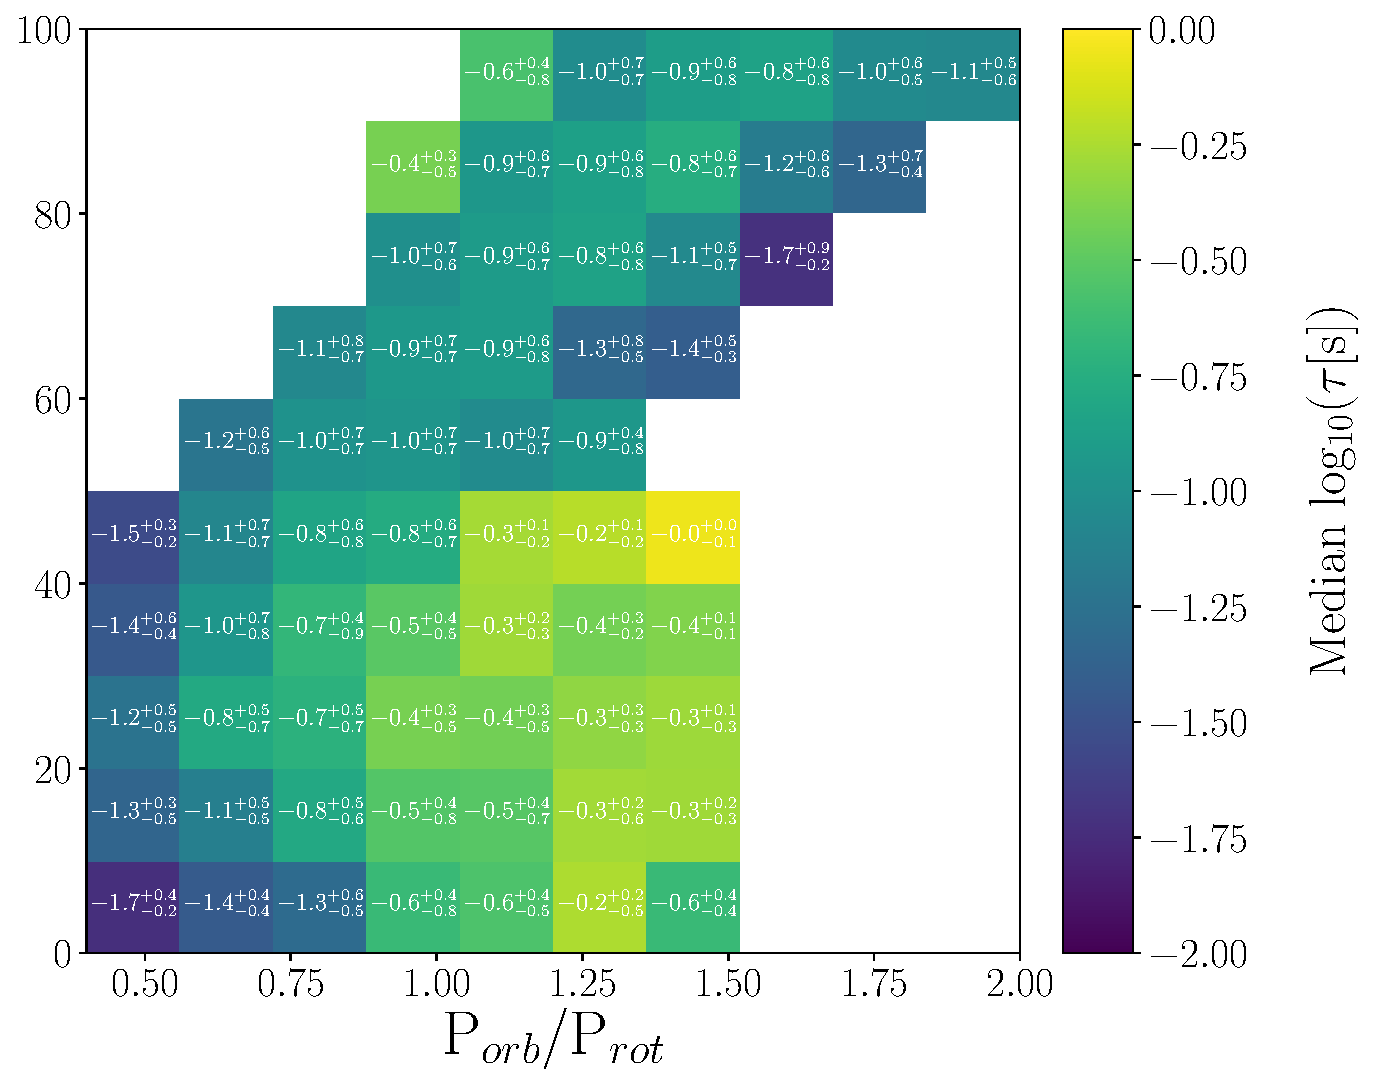
\includegraphics[width=0.45\textwidth]{../Plots/porbProtPorbTauHist.pdf}
   \caption{Same format as Fig.~\ref{fig:qmap}, but for log$_{10}(\tau [s])$ under the CTL model. }%
    \label{fig:taumap}%
\end{figure}

According to the CTL model, many binaries tidally-lock for P$_{orb} \lsim 20$ d. Tidally-locking can occur for P$_{orb} < 50$ d and $\tau \gsim 0.25$ s.  For P$_{orb} < 50$ d, subsynchronous rotation occurs for stars with $\tau < 0.1$ s as magnetic braking dominates over tidal torques.  For P$_{orb} > 50$ d, magnetic braking dominates the evolution as the diagonal sequence with a median $\tau \approx 0.1$ s has upper and lower limits that encompass most of the range we considered for $\tau$, suggesting that tides are not important in this region of parameter space.  The shape of this diagonal region arises from the combination of magnetic braking and our flat initial P$_{orb}$ distribution. We do not observe P$_{orb}/$P$_{rot} \gsim 1.5$ as we only consider eccentricities up to $e = 0.3$, limiting how rapid supersynchronous systems can rotate according to Eqn.~(\ref{eqn:ctl:eqPer}).

\subsection{P$_{rot}$ Distribution of Stellar Binaries} \label{sec:protDist}

Here we examine how the competition between tidal torques and magnetic braking shape the P$_{rot}$ distribution of low-mass stellar binaries.  We consider two cases where tidal torques dominate: ``Locked" where P$_{rot} = $ P$_{eq}$ and ``Interacting" where P$_{rot}$ is within $10\%$ of P$_{eq}$ as in this regime, tides are likely shepherding P$_{rot}$ towards the tidally-locked state keeping P$_{rot}$ close to P$_{eq}$, typically within about $10\%$ as we demonstrated in $\S$~\ref{sec:eq}, e.g. Fig.~\ref{fig:eqPer}. We refer to the remaining binaries as ``Unlocked" as magnetic braking and stellar evolution likely dominate their angular momentum evolution.  In Fig.~\ref{fig:lockedCPL} and Fig.~\ref{fig:lockedCTL}, we plot P$_{rot}$ as a function of mass for the primary stars in stellar binaries for both the CPL and CTL model, respectively, integrated to system ages uniformly sampled over $1-7$ Gyr.  

\begin{figure}
	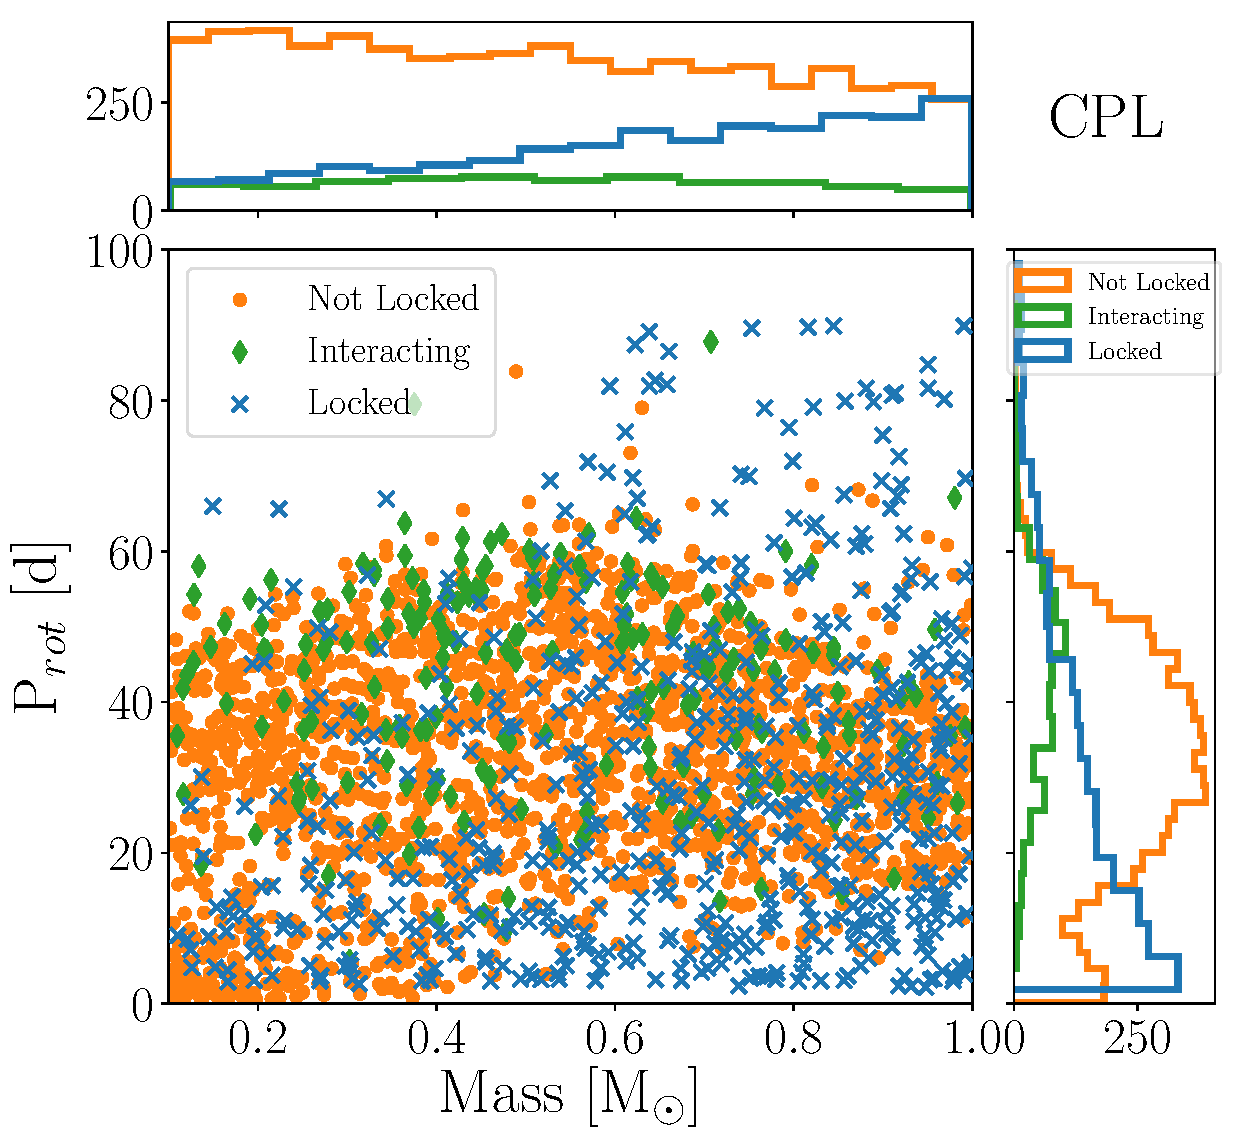
\includegraphics[width=0.45\textwidth]{../Plots/lockedCPL.pdf}
   \caption{Rotation state for tidally-locked (blue, P$_{rot} = $ P$_{eq}$), interacting (green, P$_{rot}$ within $10\%$ of P$_{eq}$ and not locked), and not locked (orange, remainder of binaries) stellar binaries. Left: P$_{rot}$ as a function of stellar mass and age according to our CPL simulations integrated to system ages uniformly sampled over $1-7$ Gyr. Right: Marginalized P$_{rot}$ distribution for each case.}%
    \label{fig:lockedCPL}%
\end{figure}

Both models predict a substantial population of tidally-locked fast rotators with P$_{rot} \lsim 20$ d, with tidally-locked stars systematically rotating faster (median CPL, CTL P$_{rot} = 27.6$ d and $7.4$ d) than unlocked (median CPL, CTL P$_{rot} = 41.3$ d and $40.8$ d) binaries. More massive stars are more likely to tidally-lock compared to less massive stars as tidal torques scale as $R^5$, and $R$ increases with stellar mass.  This feature is seen in the enhanced density of locked systems at larger masses for both tidal models, but in particular for the CPL model.

Tidal locking is not limited to P$_{orb} \lsim 20$ d, however, as we find stellar binaries can tidally-lock over a wide range of P$_{rot}$ up to P$_{rot} =$ P$_{orb} \approx 100$ d according to the CPL model, producing a slow-rotating population above the P$_{rot}$ distribution envelop of single stars. This behavior is consistent with observations of P$_{rot}$ in \kepler eclipsing binaries by \citet{Lurie2017} who find tentative evidence that binaries can tidally-lock up to their detection limit of P$_{orb} = $ P$_{rot} = 45$ d and with the observations of \citet{Abt2004}.  Under the CTL model, however, binaries predominantly tidally-lock out to only P$_{orb} \approx 20$ d, in stark contrast to the CPL model's predictions. Some binaries can tidally-lock or tidally-interact out to $P_{rot} \approx 80$ d, but not nearly as many as the CPL model, nor can the CTL model tidally-lock binaries out to P$_{orb} = 100$ d, regardless of $\tau$. Only $7.5\%$ of binaries tidally-lock according to the CTL model, compared with $25\%$ of CPL model binaries, as tidal torques are generally stronger in the CPL formalism.   

\begin{figure}
	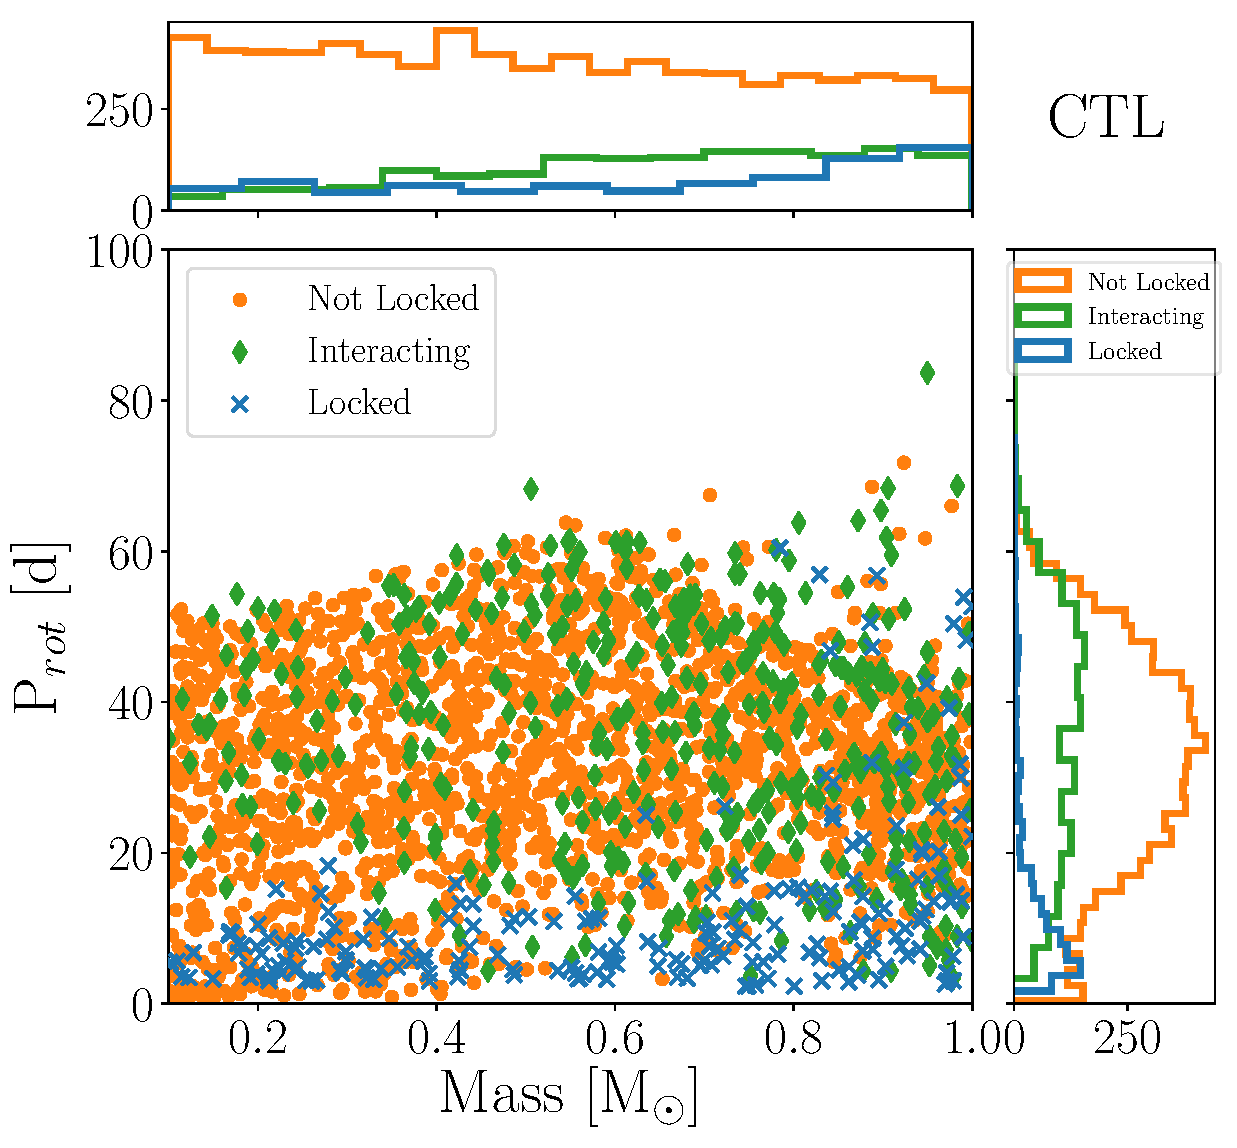
\includegraphics[width=0.45\textwidth]{../Plots/lockedCTL.pdf}
   \caption{Same format as Fig.~\ref{fig:lockedCPL}, but for the CTL simulations. }%
    \label{fig:lockedCTL}%
\end{figure}

The interacting population tends to rotate more slowly than the unlocked population as at short P$_{orb}$, and hence P$_{rot}$, binaries preferentially tidally-lock due to stronger tidal torques.  At longer P$_{orb}$, weaker tidal torques allow magnetic braking to spin down the stars past P$_{eq}$, with tidal torques eventually strengthening enough to shepherd P$_{rot}$ towards P$_{eq}$ via the mechanism discussed in $\S$~\ref{sec:eq}. The CPL and CTL models predict that $34\%$ and $25\%$ of stars, respectively, are either tidally-locked or interacting, demonstrating that tidal torques play a pivotal role in shaping the angular momentum evolution in stellar binaries across a wide range of parameters. The P$_{rot}$ - mass distribution for unlocked binaries resembles the single star sequence observed in the center right panel of Fig.~\ref{fig:protDist} indicating that magnetic braking and stellar evolution dictate their angular momentum evolution as expected.

\begin{figure}
	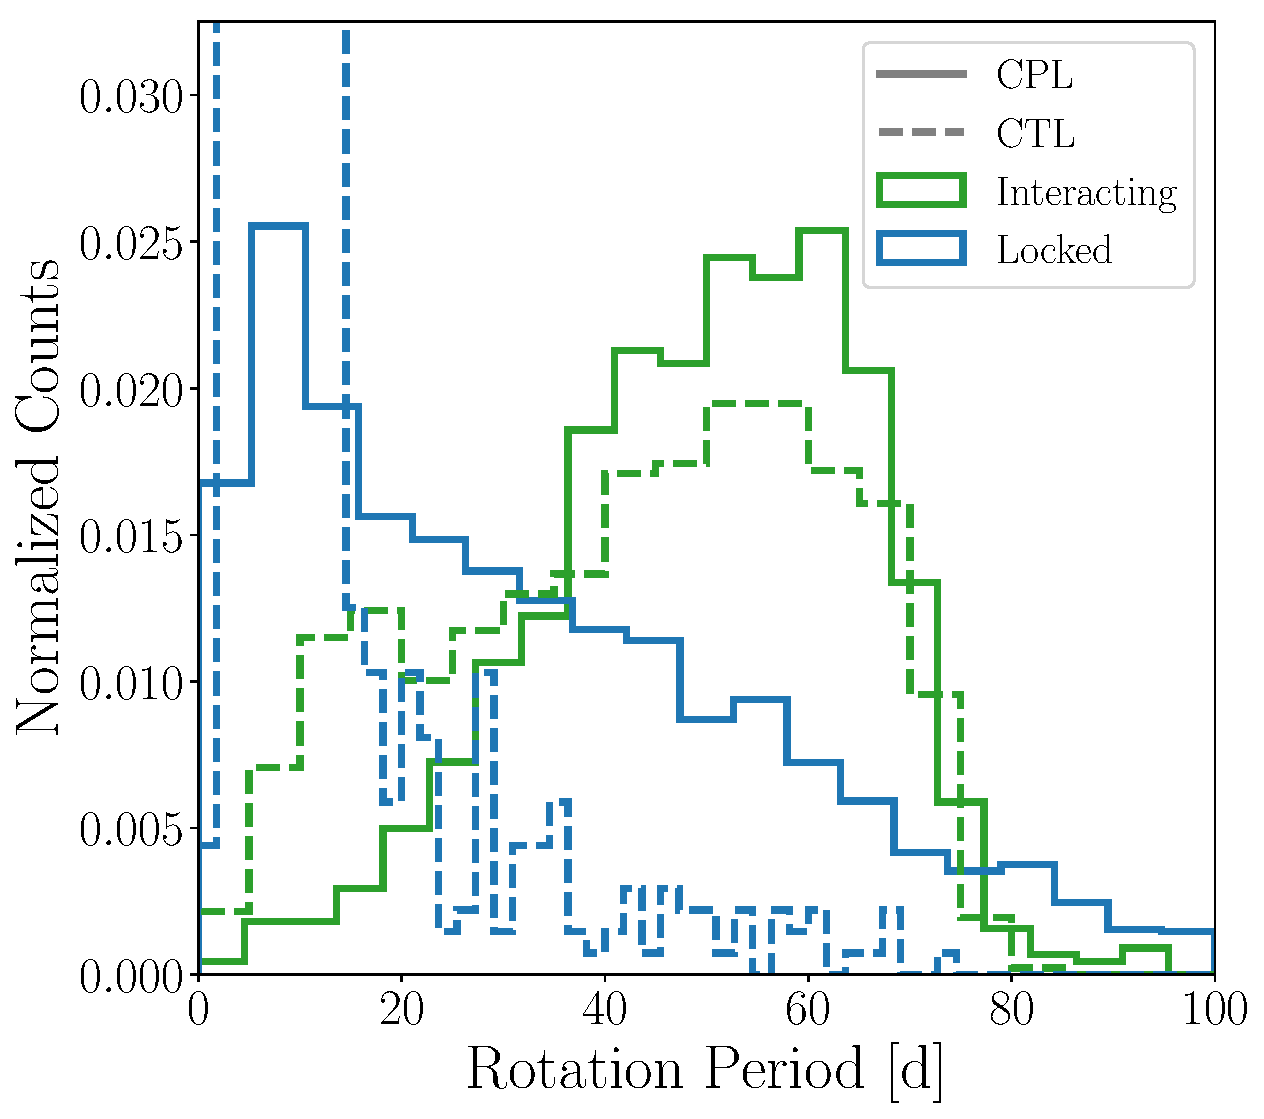
\includegraphics[width=0.45\textwidth]{../Plots/lockedProtHist.pdf}
   \caption{P$_{rot}$ distribution for tidally-locked (blue) and interacting (green, P$_{rot}$ within $10\%$ of P$_{eq}$ and not locked) binaries according to the CPL (solid line) and CTL (dashed line) models.}%
    \label{fig:lockedProtHist}%
\end{figure}

As shown in Fig.~\ref{fig:lockedProtHist}, both models predict that tidal torques can influence the P$_{rot}$ evolution out to P$_{orb} \approx 80$ d, causing a significant departure from the long-term expected spin down of single stars due to magnetic braking.  The CTL model predicts that the majority tidally-locked binaries, $86\%$, lock into rapid rotation with P$_{rot} \lsim 20$ d, typically in short P$_{orb}$ binaries where tidal torques are strongest as the median locked CTL P$_{orb} = 7.6$ d. The CPL model, however predicts that binaries can tidally-lock into a wide range of rotation states with only $39\%$ of locking binaries have P$_{rot} < 20$ d, while many lock out to P$_{rot} \approx 100$ d, with the latter state corresponding to tidal synchronization in long P$_{orb}$ binaries.  The presence of P$_{orb} > 20$ d locked population, or lack there of, could be a powerful observational discriminant between which equilibrium tidal model acts in low-mass stellar binaries.  We discuss this point further in $\S$~\ref{sec:whichModel}.

\subsection{Deviations From Single Star P$_{rot}$ Evolution: Implications for Gyrochronology} \label{sec:gyro}

We compare the P$_{rot}$ distribution for tidally-interacting stellar binaries from our CPL and CTL simulations with the P$_{rot}$ distribution of single stars subject to stellar evolution and magnetic braking to gauge the impact of tidal torques on driving P$_{rot}$ distributions away from that of single stars.  We simulate 10,000 single star systems according to the evolution described in $\S$~\ref{sec:methods:stellar} with initial conditions sampled from the same mass and P$_{rot}$ distributions used for the binary simulations described $\S$~\ref{sec:methods}. In Fig.~\ref{fig:protDist}, we display P$_{rot}$ as a function of mass and age for binaries simulated using both the CPL and CTL model and for single stars. We perform this procedure for stars losing angular momentum via magnetic braking according to both the \citet{Matt2015} and \citet{Reiners2012} magnetic braking models.

\subsubsection{\citet{Matt2015} Magnetic Braking}

% In the absence of external forces, the long-term P$_{rot}$ evolution of low-mass stars is governed by magnetic braking.  In stellar binaries, however, tidal torques compete against magnetic braking to drive P$_{rot}$ towards P$_{eq}$, e.g. Fig.~\ref{fig:eqPer}, causing their P$_{rot}$ evolution to differ from that of a single star.  Here w

\begin{figure*}[t]
	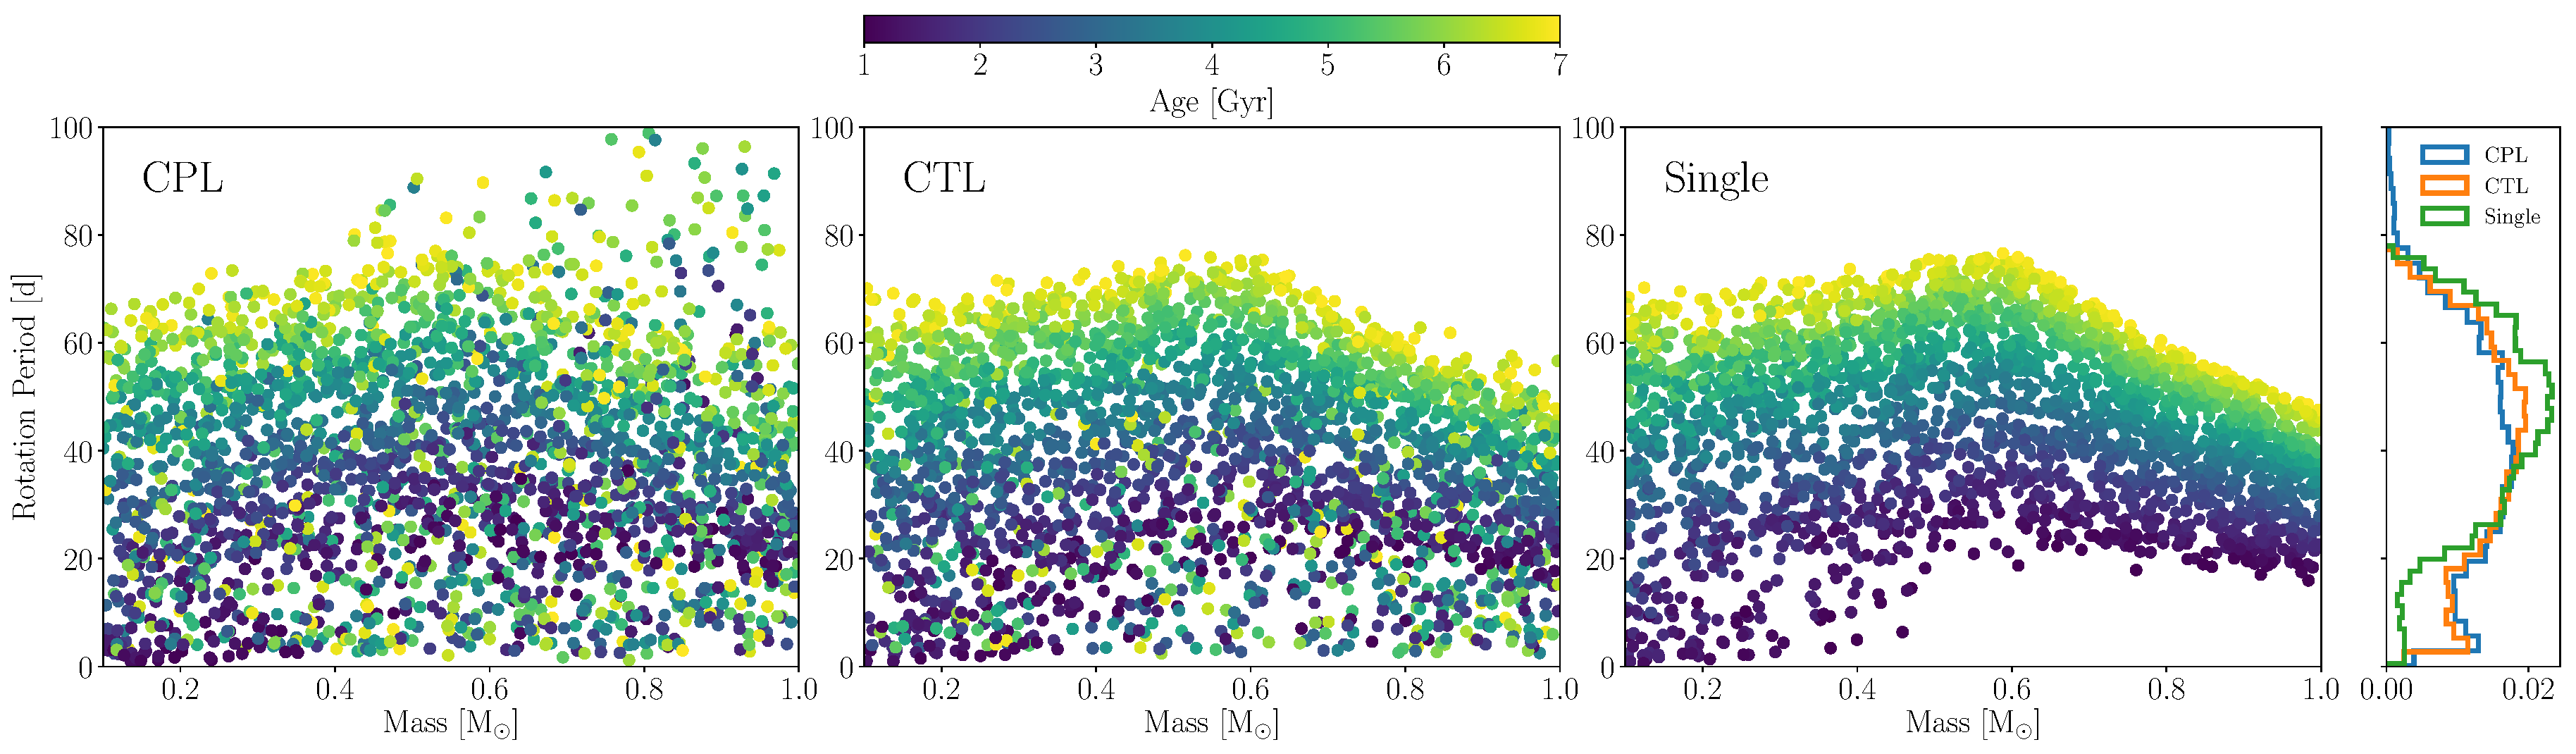
\includegraphics[width=\textwidth]{../Plots/protDist.pdf}
   \caption{P$_{rot}$ as a function of stellar mass and age according to our CPL (left), CTL (left center), and single star (right center) simulations integrated to system ages uniformly sampled over $1-7$ Gyr using the \citet{Matt2015} magnetic braking model. For each case, we only plot 2,500 systems for clarity but account for all systems when computing the marginalized distributions. Right: The P$_{rot}$ distribution for each case, marginalized over stellar mass.}%
    \label{fig:protDist}%
\end{figure*}

There is a clear age-dependence of P$_{rot}$ seen in the single star population with older stars rotating more slowly, a trend that is borne out in nature and is the critical assumption of gyrochronology methods that link P$_{rot}$ to stellar ages via the magnetic braking-driven long-term spin down of low-mass stars \citep[e.g.][]{Skumanich1972,Barnes2003,Barnes2007,Mamajek2008,Barnes2010,Meibom2015}. The only rapidly rotating single stars are young (ages $< 2$ Gyr) M dwarfs (M$ < 0.5$ M$_{\odot}$) have just reached the main sequence and have not yet experienced substantial angular momentum loss due to magnetic braking.  In stark contrast, both tidal models predict a substantial population of tidally-locked fast rotators (P$_{rot} < 20$ d). Under the CPL and CTL models, $18\%$ and $19\%$ of simulated stars have P$_{rot} < 20 $ d, respectively, compared to only $5\%$ in the single star models.  At the long P$_{rot}$ end, the CPL model predicts a population of slow rotators with P$_{rot} \gsim 70$ d, a feature not seen in either the CTL or single star models, and is produces by tidal-locking in long P$_{orb}$ binaries with low tidal $Qs$, e.g. Fig.~\ref{fig:lockedCPL}.

Both tidal models predict that age does not strongly correlate with P$_{rot}$ in low-mass binaries, especially for P$_{rot} < 20 $ d, as many of these systems tidally-lock at short P$_{orb}$. The median ages and $68\%$ interval for fast rotators (P$_{rot} \lsim 20$ d) are $2.8^{+2.9}_{-1.5}$ Gyr and $3.1^{+2.6}_{-1.8}$ Gyr according to the CPL and CTL models, respectfully, compared to much younger single stars with ages of $1.3^{+0.5}_{-0.3}$ Gyr. We highlight this point in Fig.~\ref{fig:protAgeHist} by plotting a histogram of system ages from Fig.~\ref{fig:protDist} for single or primary stars in binaries with P$_{rot} < 20$ d.  

\begin{figure}[h]
	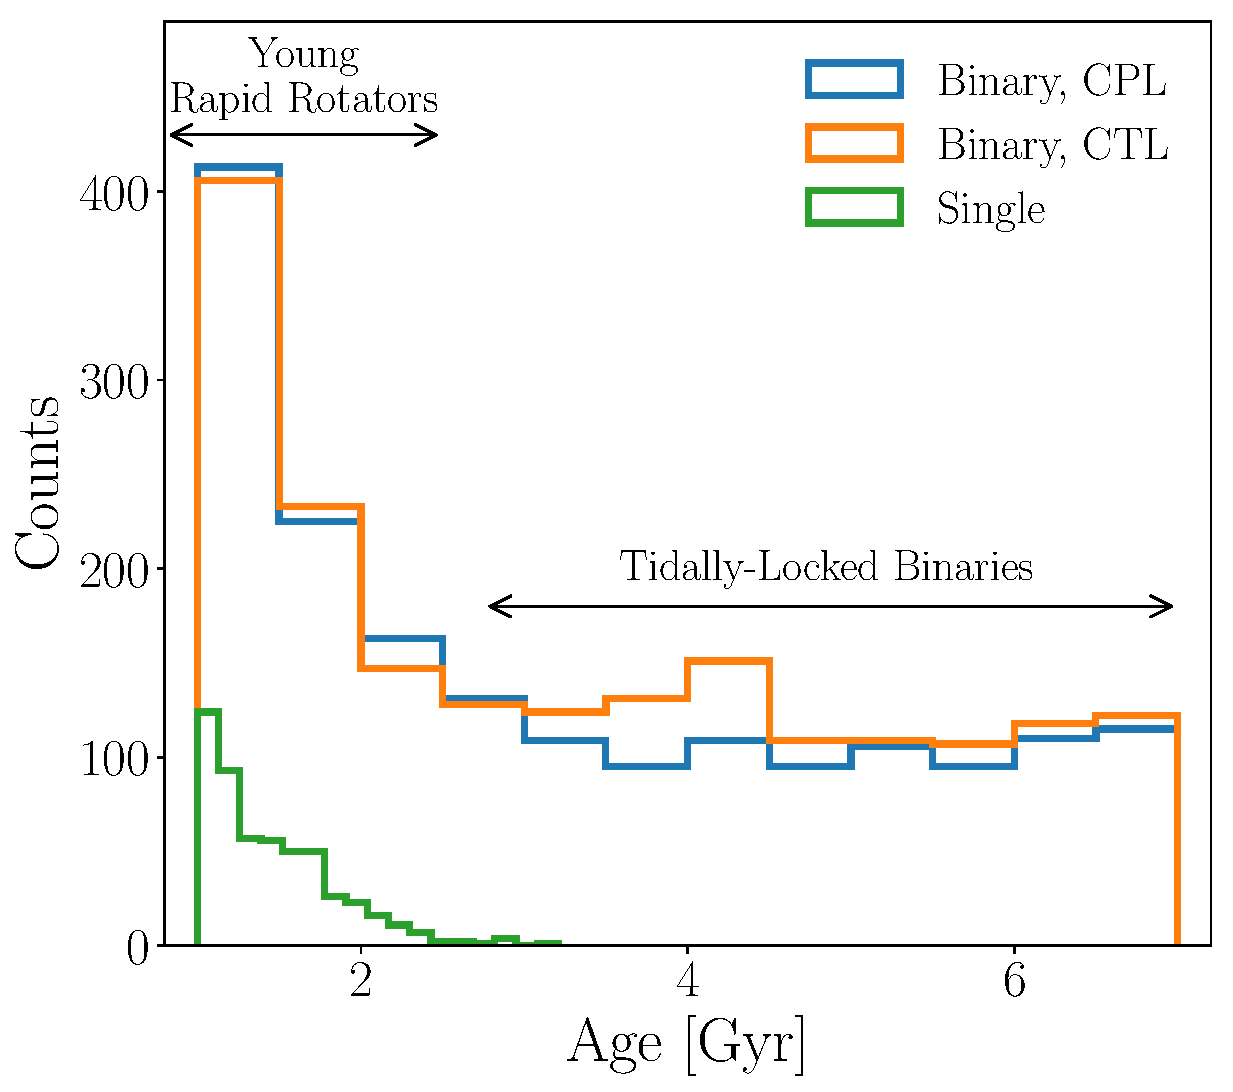
\includegraphics[width=0.45\textwidth]{../Plots/protAgeHist.pdf}
   \caption{Histogram of rapidly-rotating (P$_{rot} < 20$ d) stellar ages for single and primary stars in binaries from Fig.~\ref{fig:protDist}. Rapidly-rotating single stars must be young (ages $\lsim 2$ Gyr), while tidally-locked rapidly-rotating binaries exhibit a wide range of ages.}%
    \label{fig:protAgeHist}%
\end{figure}

\subsubsection{\citet{Reiners2012} Magnetic Braking}

Similar to the \citet{Matt2015} simulations discussed above, the single star simulations display a clear age-dependence of P$_{rot}$. The \citet{Reiners2012} model's magnetic braking transition at $M = 0.35$ M$_{\odot}$ produces a sharp cutoff in the P$_{rot} - M$ distribution between late M dwarfs and more massive stars.  More massive stars ($M \geq 0.35$ M$_{\odot}$) follow a smooth P$_{rot} -$ age sequence, while the late M dwarfs can remain rapidly rotating if they are young and in the saturated regime or extremely slowly rotating if the are older than about 4 Gyr. As in the \citet{Matt2015} model, the only rapid rotators (P$_{rot} \lsim 20$ d) are very young stars with ages $\lsim 2$ Gyr. The presence of extremely slowly rotating late M dwarfs, absent in the predictions of the \citet{Matt2015} model but seemingly present in nature \citep[e.g.][]{Newton2018}, could be used as an observational discriminant between the \citet{Matt2015} and \citet{Reiners2012} model, but a full investigation of which magnetic braking model accurately describes angular momentum loss in low mass stars is beyond the scope of this work. 

\begin{figure*}[t]
	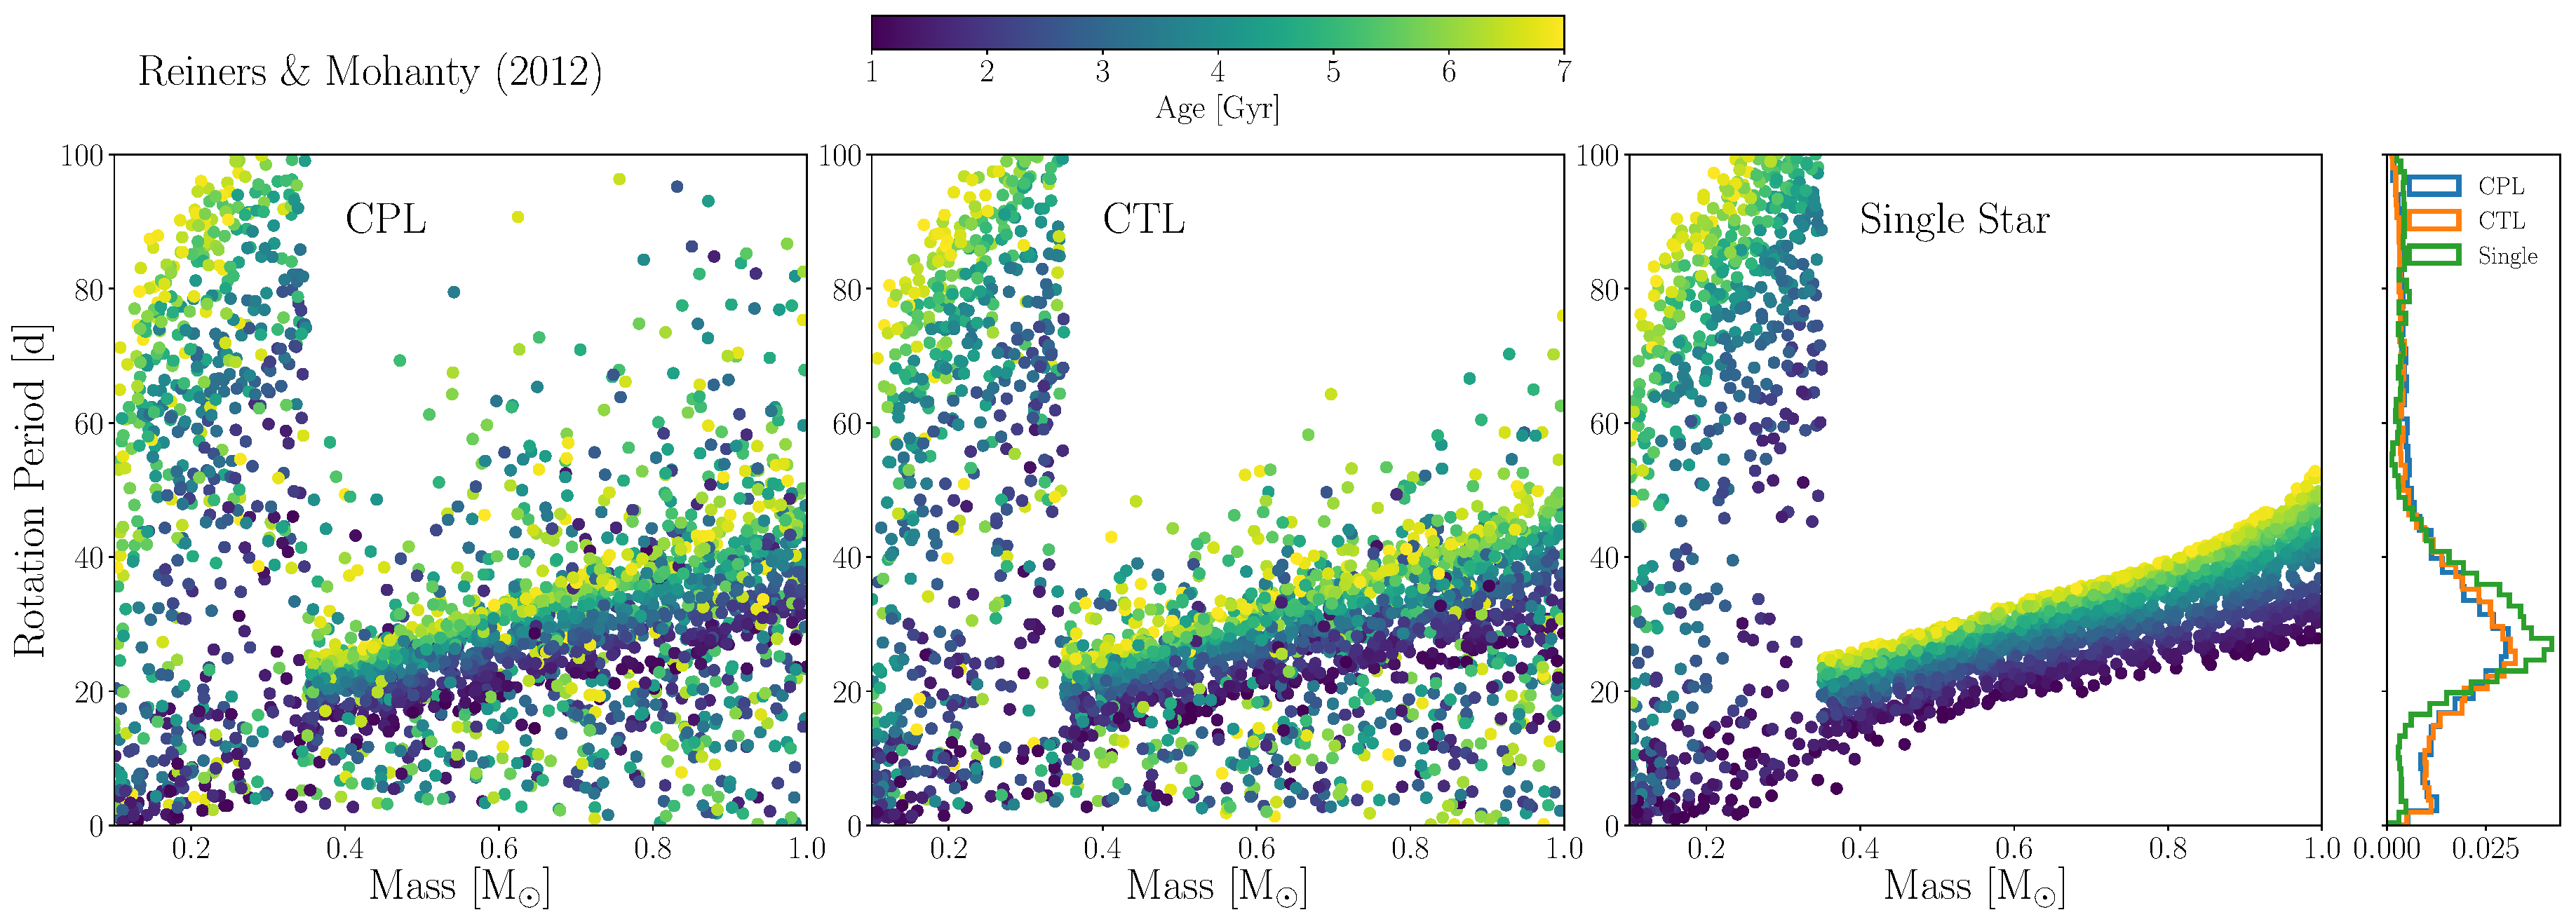
\includegraphics[width=\textwidth]{../Plots/protDistReiners.pdf}
   \caption{Same format as Fig.~\ref{fig:protDist}, but evolved using the \citet{Reiners2012} magnetic braking model.}%
    \label{fig:protDistReiners}%
\end{figure*}

The general trends found in the coupled stellar-tidal simulations using the \citet{Matt2015} model persist in the simulations evolved using the \citet{Reiners2012} model, demonstrating that these findings are not magnetic braking model-dependant, but rather a generic result of the interaction between magnetic braking and tidal torques in low-mass binaries. Both the CPL and CTL simulations display a clear single-star magnetic braking-dominated sequence, but as before, tidally-locked binaries appear across a wide range of P$_{rot}$ and primary star masses. Both the CPL and CTL model tidally-lock many short P$_{orb}$ stars into rapid rotation across all masses, with both models predicting $23\%$ of stars have P$_{rot} < 20$ d, compared to $11\%$ of single-stars, mostly for late M dwarfs in the latter case. As shown above, the CTL model predicts that binaries can strongly tidally-interact out to long P$_{orb}$, seen out to P$_{rot} = 80$ d, while the CPL model can tidally-lock stars out to P$_{orb} \approx 100$ d. These strong tidal interactions decouple P$_{rot}$ from age in binaries, mirroring the behavior discussed above, especially for rapid rotators. The median ages and $68\%$ interval for fast rotators (P$_{rot} \lsim 20$ d) are $2.6^{+2.8}_{-1.3}$ Gyr and $2.7^{+2.7}_{-1.4}$ Gyr according to the CPL and CTL models, respectfully, compared to much younger single stars with ages of $1.7^{+0.9}_{-0.5}$ Gyr, similar to the age distributions for rapid rotators evolved using the \citet{Matt2015} model.   

\subsubsection{Impact of Binarity on Gyrochronology}

Tidal torques pose a fundamental problem for inferring ages of stars via gyrochronlogy. Regardless of the choice of equilibrium tidal model or magnetic braking model, stellar binaries readily tidally-lock, or at least strongly tidally-interact, across a wide range of P$_{orb}$ and primary star masses, decoupling P$_{rot}$ from age. For example, if one observed a rapidly rotating star with P$_{rot} \lsim 20$ d, gyrochronology models would predict ages $\lsim 2$ Gyr. If a rapidly-rotating star is actually an unresolved binary, it would likely be tidally-locked, decoupling P$_{rot}$ from age, causing the predictions of gyrochronology models to fail as its age could be at least several Gyrs, e.g. Fig.~\ref{fig:protAgeHist}. This effect is most likely to manifest in rapid rotators (P$_{rot} < 20$ d), but persists across all P$_{rot}$ up to 100 d, producing a significant contaminating signal, e.g. Fig.~\ref{fig:protDist} and Fig.~\ref{fig:protDistReiners}. 

In general, it is difficult to accurately determine if a source is single star or a stellar binary via longterm photometric monitoring as only a small fraction of stars in binaries will occult one another. Observations of the binarity of field stars by \citet{Raghavan2010} and \citet{Duchene2013} indicate that roughly half of stars are in stellar binaries, with $10\%$ of these binaries having P$_{orb} \lsim 100$ d, suggesting that unless one accounts for binarity, stellar binaries will produce a non-negligible contaminating signal in any study of stellar rotation periods and any ages inferred via gyrochronlogy are potentially subject to large systematic errors.  Moreover, this problem could be more significant than the aforementioned estimate implies as \citet{Simonian2018} found that most rapid rotators with P$_{rot} \leq 7.5$ d in the \kepler field are likely photometric binaries, suggesting that binary contamination in P$_{rot}$ studies could be widespread. We caution that any application of gyrochronlogy methods to predict ages for stars, especially those with P$_{rot} \lsim 20$ d, should rule out or account for stellar binarity, or otherwise risk deriving systematically incorrect ages.

Furthermore, any study of the angular momentum evolution of a stellar population will be flawed unless one robustly accounts for binarity.  Tidal torques do not just produce spin-orbit synchronization at short P$_{orb}$, but can produce a rich variety of rotation states that deviate from the expected long-term spin-down experienced by single stars, e.g. Fig.~\ref{fig:qmap} and Fig.~\ref{fig:taumap}. We recommend that the application of or the calibration of magnetic braking models to a sample of stellar rotation periods control for binarity.   

% In binaries, however, tidal torques can lock stellar P$_{rot}$ to P$_{eq}$, especially at short P$_{orb}$ where tidal torques are stronger, creating a long-lasting population of fast rotators with a wide age range. 
% This feature is not due to long-term spin-down via magnetic braking as this population lies above the old edge of single star sequence. Instead 

%% SECTION: COMPARISON TO KEPLER %%
\subsection{Comparison to \kepler} \label{sec:kepler}

We compare our simulation results using both tidal models and the \citet{Matt2015} magnetic braking model to P$_{rot}$ measurements of primary stars in \kepler low-mass eclipsing stellar binaries by \citet{Lurie2017}.  \citet{Lurie2017} measured 816 rotation periods for primary stars in \kepler EBs with starspot modulations and visually inspected each light curve to ensure their accuracy. The \citet{Lurie2017} dataset is the largest homogenous set of P$_{rot}$ measurements available for low-mass stellar binaries and represents the state of the art benchmark for studies of the influence of tides on P$_{rot}$ in stellar binaries. We compare our results to the P$_{1,min}$ P$_{rot}$ values reported by \citet{Lurie2017} as the authors demonstrated that these values are likely to be close to the equatorial P$_{rot}$ that we track in our simulations.

In Fig.~\ref{fig:lurie7}, we display P$_{orb}/$P$_{rot}$ as a function of P$_{orb}$ for both the CPL and CTL models where each simulation was integrated to an age uniformly sampled over $1-7$ Gyr, consistent with ages of \kepler field stars \citep{Chaplin2014}.  Both models qualitatively reproduce most trends in the \citet{Lurie2017} data, namely the large cluster of synchronized rotators and the population of subsynchronous rotators, both for P$_{orb} \lsim 20$ d. Magnetic braking and age imparts two noticeable features in the data. First, supersynchronous rotators with P$_{orb}/$P$_{rot} > 1.5$, especially at long P$_{orb}$, corresponds to young stars that have yet to significantly spin down due to magnetic braking or tides.  Second, the lower limit seen in both panels is a line of nearly constant P$_{rot} \approx 60$ d set by how much a star can spin down via magnetic braking in the weak tides regime over 7 Gyr, the longest age considered in our simulations.  

\begin{figure*}[t]
	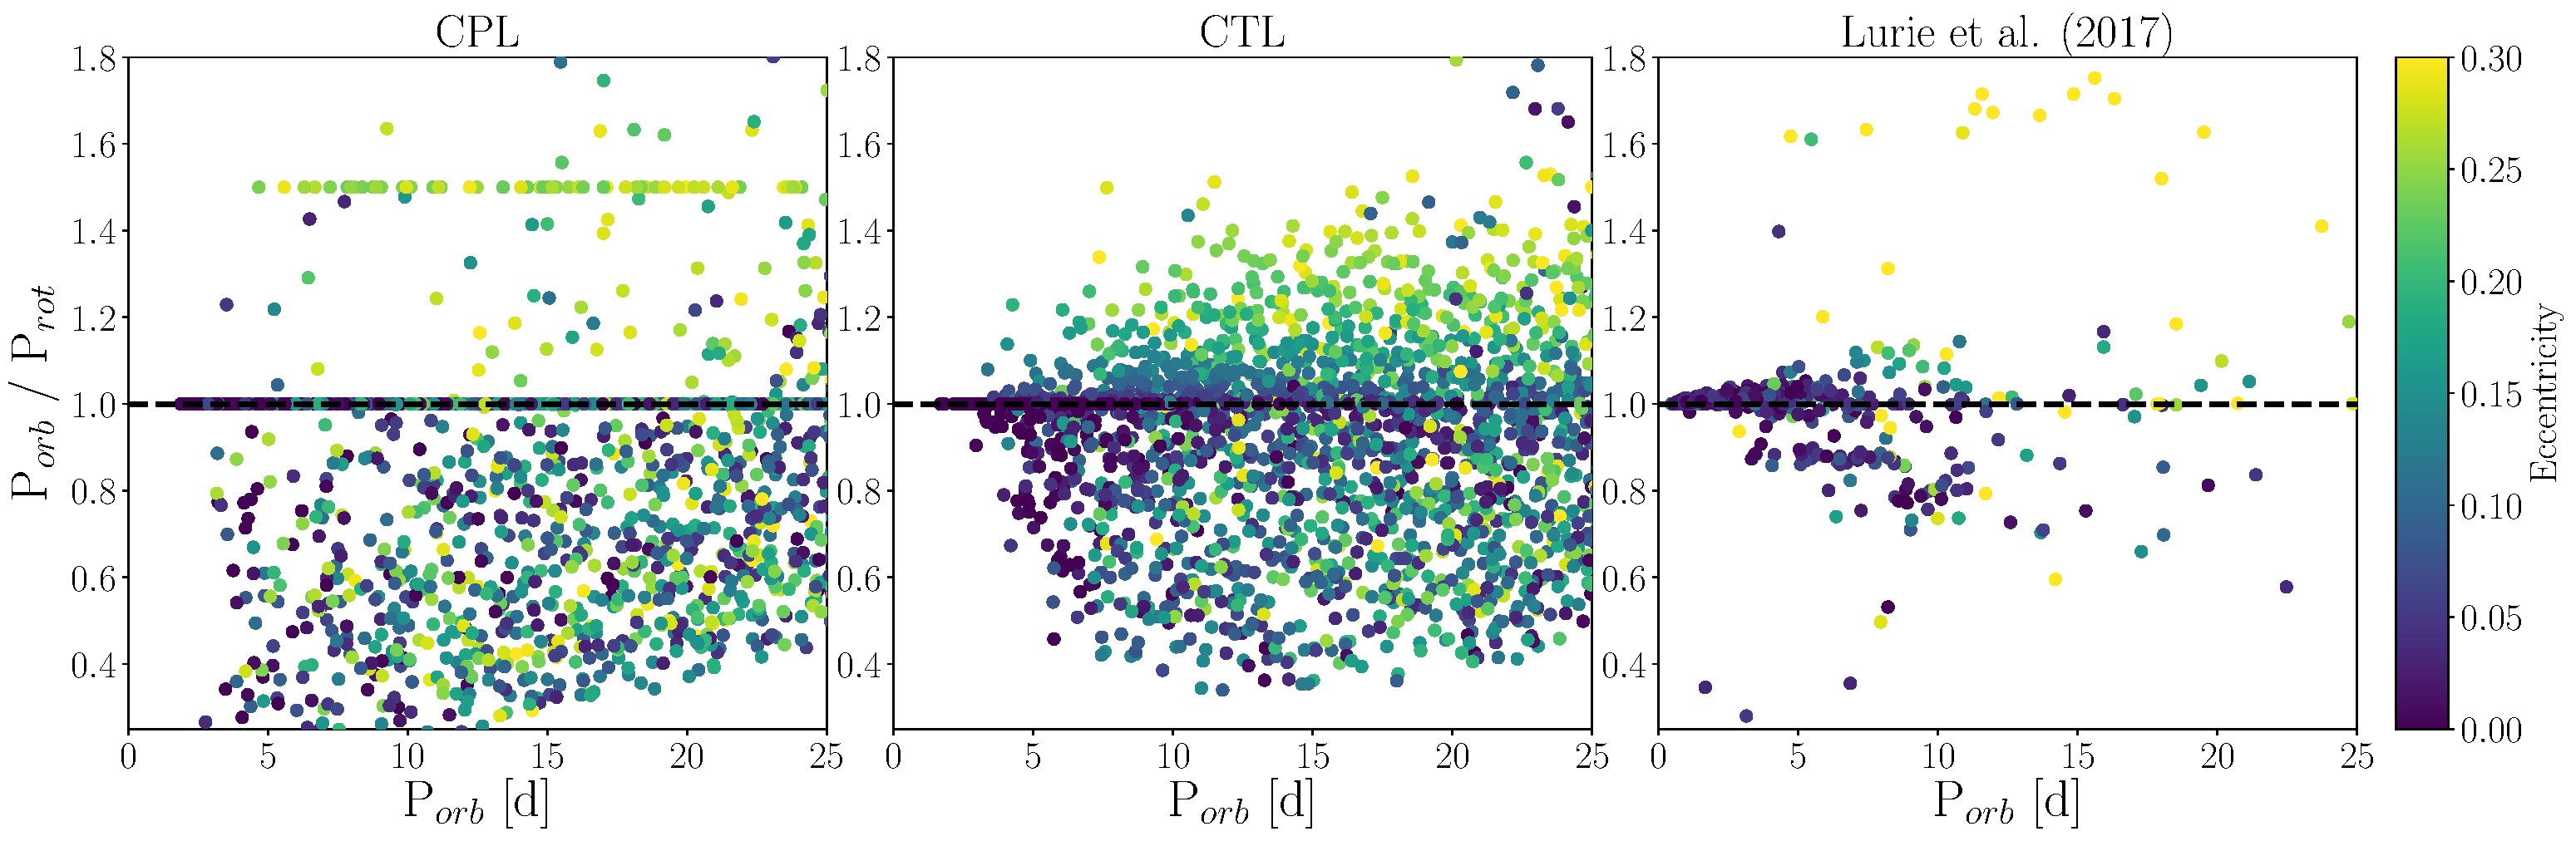
\includegraphics[width=\textwidth]{../Plots/lurieFig7.pdf}
   \caption{P$_{orb}/$P$_{rot}$ as a function of P$_{orb}$ simulated according to the CPL model (left) and the CTL model (right) colored by $e$, compared with \kepler EBs from \citet{Lurie2017} (red plus signs).  The \kepler EBs at low P$_{orb}$ and low P$_{orb}/$P$_{rot}$ are likely either brown dwarfs or exoplanets \citep{Lurie2017}, and hence not modeled by our simulations, so we do not consider them, but we display them for completeness.}%
    \label{fig:lurie7}%
\end{figure*}

Both models can reproduce the major trends in the data, but the predictions of the CPL model fail to reproduce several key aspects.  First, the CPL model cannot reproduce the cluster of supersynchronous rotators with P$_{orb}/$P$_{rot} \lsim 1.1$ for P$_{orb} < 10$ d and instead predicts that all tidally-locked sypersynchronous rotators lie on the line P$_{orb}/$P$_{rot} = 1.5$.  This prediction is inconsistent with the data as no obvious spin-orbit commensurablity, aside from 1:1 synchronization, is present in the data, likely because stellar convective envelopes lack a fixed shape, making resonant coupling difficult unless coupling occurs with internal gravity or pressure modes \citep{Burkart2014,Lurie2017}.  The CPL model can produce the population of subsynchronous rotators observed for $10 \lsim$ P$_{orb} \lsim 20$ d, but fails to produce the prominent cluster of subsynchronous rotators at P$_{orb}/$P$_{rot} \approx 0.9$ for P$_{orb} < 10$ d observed by \citet{Lurie2017}.  The CTL model, however, seems to excel where the CPL models fails by qualitatively reproducing both populations. We examine these features further by comparing results from our CTL model with the \citet{Lurie2017} data where the data is most complete, P$_{orb} < 10$ d, in $\S$~\ref{sec:subsync}, and offer tests to discriminate between the two models in $\S$~\ref{sec:whichModel}. 

\subsubsection{P$_{orb} < 10$ d According to the CTL Model} \label{sec:subsync}

Our coupled stellar-tidal model reproduces many of the the spin and orbital features seen in low-mass \kepler EBs when using the CTL formalism. In Fig.~\ref{fig:subsync}, we compare our simulated systems (dots) with the observed \citet{Lurie2017} EB data (crosses), where both points are colored by $e$. \citet{Lurie2017} find that $15\%$ of their subsynchronous population with 2 $< P_{orb} <$ 10 days has P$_{orb}/$P$_{rot} \in [0.84, 0.92]$, the cluster of stars those authors identified near $P_{orb}/$P$_{rot} = 0.9$, compared with $9\%$ of our CTL population, suggesting that subsynchronous rotation is a common outcome of stellar-tidal evolution in low-mass binaries. Furthermore in the same P$_{orb}$ regime, \citet{Lurie2017} find that $72\%$ of their population has P$_{orb}/$P$_{rot} \in [0.92, 1.2]$, compared with $72\%$ of our CTL population, in good agreement. In comparison, the CPL model (not pictured) predicts $68\%$ of the population has P$_{orb}/$P$_{rot} \in [0.92, 1.2]$ and $2\%$ has P$_{orb}/$P$_{rot} \in [0.84, 0.92]$ for 2 $< P_{orb} < $ 10 d, producing a population of synchronized binaries similar to what is seen in the \kepler EB population, but not the subsynchronous cluster identified by \citet{Lurie2017}.   

Nearly all simulated binaries with P$_{orb} < 4$ d have circularized orbits and synchronized spins due to strong tidal torques at short stellar separations, in excellent agreement with the \citet{Lurie2017} observations. At very short P$_{orb}$ in the absence of a perturbing tertiary companion, circularization and synchronization is the inevitable end state for low-mass binaries.  Beyond P$_{orb} \approx 4$ d, tidally-locked, eccentric binaries populate the supersynchronous population, again in excellent agreement with the \citet{Lurie2017} \kepler data.  These systems have tidally-locked but their orbits have not yet circularized, even though they likely experience strong tidal torques at short separations, because the tidal locking time scale is 2-3 orders of magnitude less than the circularization timescale \citep{Mazeh2008}.

\begin{figure}
	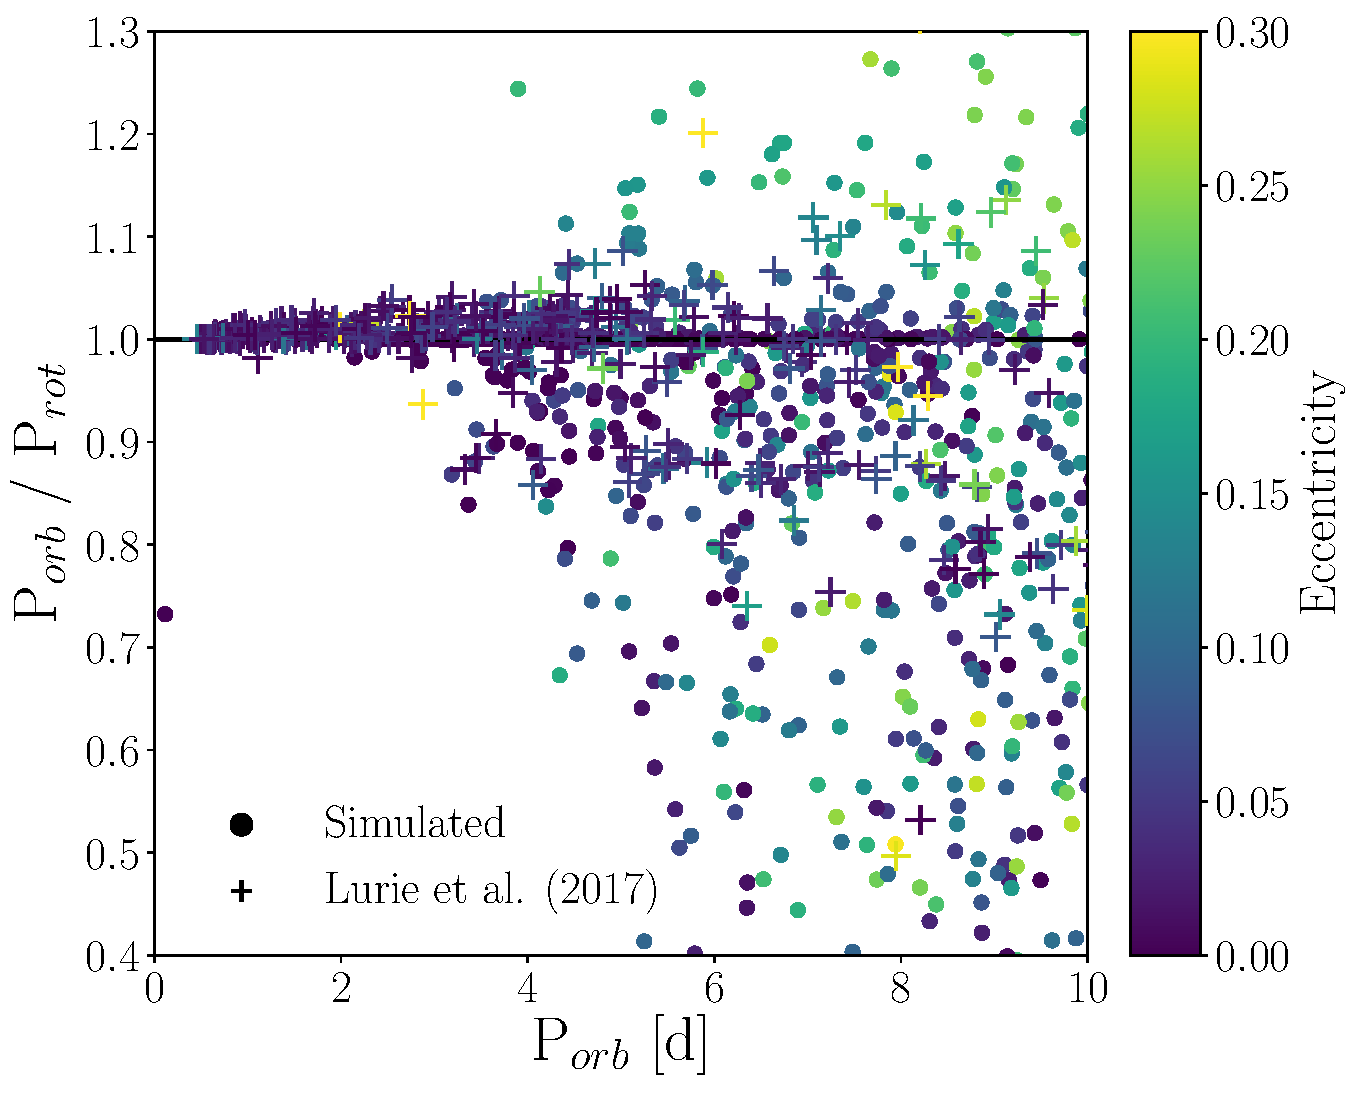
\includegraphics[width=0.45\textwidth]{../Plots/subsync.pdf}
   \caption{Same format as Fig.~\ref{fig:lurie7}, with \citet{Lurie2017} data plotted as crosses.  All points are colored according to the binary orbital $e$. Our simulations reproduce many of the observed orbital and rotational features seen in the \kepler EB population.}%
    \label{fig:subsync}%
\end{figure}

For P$_{orb} \gsim 4$ d, our model produces a population of subsynchronous rotators, including a cluster of subsynchronously rotating stellar binaries with nearly circular orbits. Although \citet{Lurie2017} argues that differential rotation creates the subsynchronous population, we find that the competition between weak tidal torques and magnetic braking described in $\S$~\ref{sec:eq} naturally produces subsynchronous rotators.  Our simulated subsynchronous binaries have systematically weaker tidal torques than the rest of the sample, as expected, as they have a median $\tau = 0.17$ s, compared to the median $\tau = 0.47$ s for the tidally-locked supersynchronous population.  
Our simulations can qualitatively reproduce many features seen in the \citet{Lurie2017} \kepler data, indicating that the equilibrium tide formalism can successfully model the tidal evolution of low-mass stellar binaries, especially at short P$_{orb}$. The comparison between theory and observations, however, is limited to more qualitative comparisons for two reasons.  First, the \citet{Lurie2017} P$_{rot}$ data lack uncertainties and \citet{Lurie2017} used transit durations and ingress/egress times to approximate the EB orbital $e$, leading to inaccurate $e$ determinations. In the absence of more accurate constraints in the \citet{Lurie2017} \kepler data, we cannot robustly compare out simulation results with observations to discriminate between which equilibrium tidal model better describes tidal torques in low-mass. Second, without reliable and accurate prior distributions for unconstrained quantities like $Q$, $\tau$, and the initial P$_{orb}$, it is difficult to perform a true Monte Carlo study that would allow us to directly compare our simulated distributions to the observations. The lack of good priors and accurate data inhibits us from conditioning our model on the observed data to infer properties such as $Q$ and $\tau$, perhaps as a function of mass, but still permits us to qualitatively compare our results with observations and demonstrate how our model can reproduce most features seen in the data.  We discuss this point further in $\S$~\ref{sec:inference}.

%\subsubsection{$Q$, $\tau$ Constraints from P$_{orb}$ and P$_{rot}$} \label{sec:qTau}

%In $\S$~\ref{sec:qTauMaps}, we demonstrated that certain rotation states typically occur for a limited subset of tidal parameters.  For example for a low-mass short P$_{orb}$ stellar binary, if we observe subsynchronous rotation, we can infer that tidal torques must be weak since magnetic braking dominates the P$_{rot}$ evolution, implying that those stars have large $Q$ or small $\tau$, as demonstrated in Fig.~\ref{fig:qmap} and Fig.~\ref{fig:taumap}. By measuring P$_{rot}$ for the primary star in a stellar binary and P$_{orb}$, one can therefore constrain the strength of the tidal interaction that led to that rotation state.  Here, we compare \kepler EB spin-orbital states measured by \citet{Lurie2017} with our simulation results to derive approximate constraints on the tidal model parameters, $Q$ and $\tau$.  
%We assign each binary in the \citet{Lurie2017} dataset to its corresponding P$_{orb}$, P$_{orb}/$P$_{rot}$ bin in in Fig.~\ref{fig:qmap} and Fig.~\ref{fig:taumap} and draw 100 samples of $Q$ and $\tau$, with replacement, from our simulated CPL and CTL model data, respectively, in the same bin to build approximate $Q$ and $\tau$ distribution for each system.  We combine the $Q$ and $\tau$ distributions, respectively, for all binaries in the \citet{Lurie2017} data to produce approximate distributions for $Q$ and $\tau$, marginalized over all other parameters, and display them in Fig.~\ref{fig:qLurie} and Fig.~\ref{fig:tauLurie}.

%\begin{figure}
%	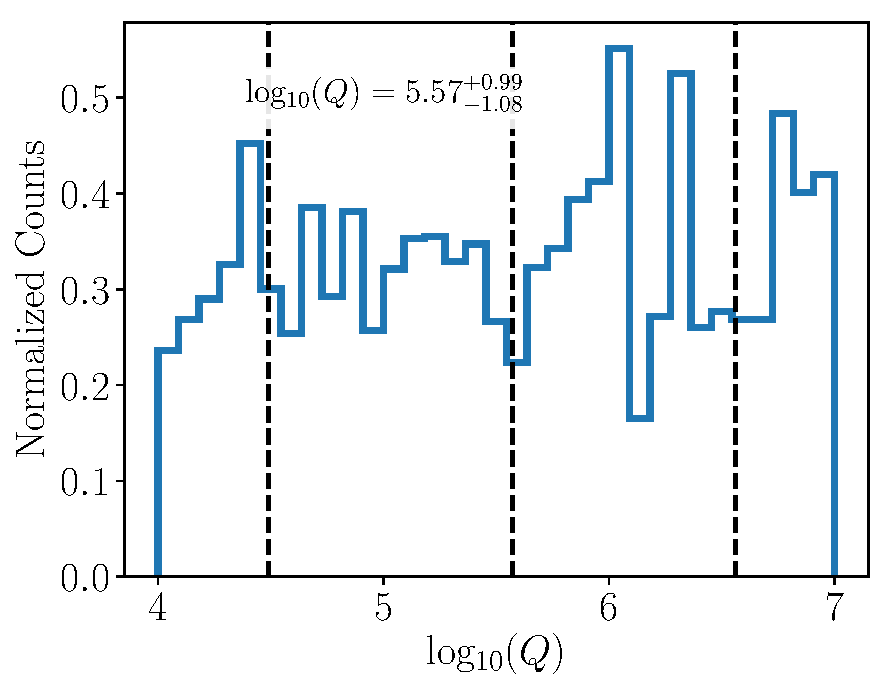
\includegraphics[width=0.45\textwidth]{../Plots/qLurie.pdf}
%   \caption{Distribution of stellar tidal $Q$ produced by convolving \citet{Lurie2017} observations of EBs' P$_{rot}$ and P$_{orb}$ with our CPL simulation results shown in Fig.~\ref{fig:qmap}. The dashed black lines, from left to right, indicate the $16^{th}$ percentile, median, and $84^{th}$ percentile.}%
%    \label{fig:qLurie}%
%\end{figure}

%\begin{figure}
%	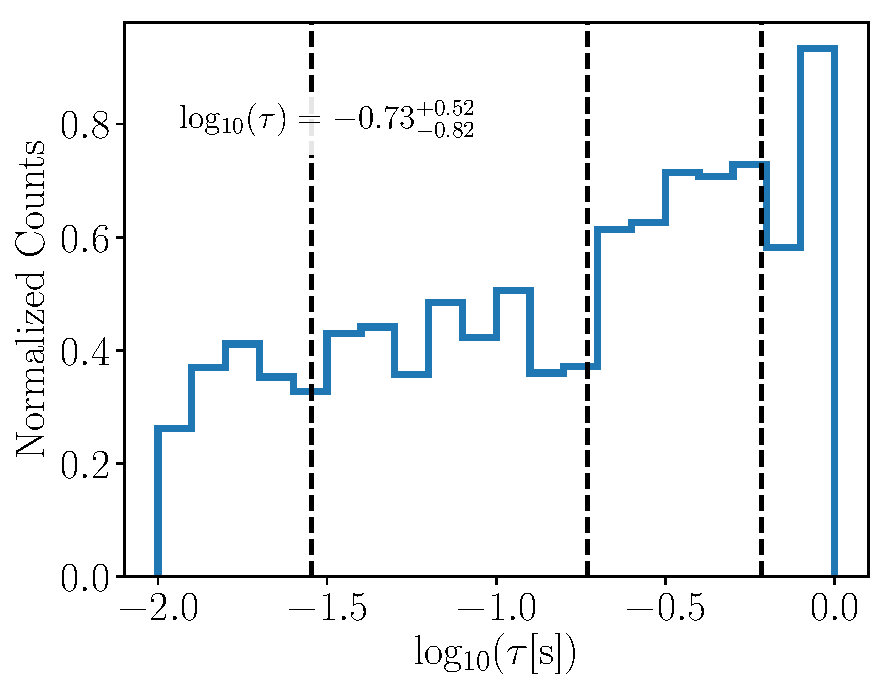
\includegraphics[width=0.45\textwidth]{../Plots/tauLurie.pdf}
%   \caption{Same as Fig.~\ref{fig:qLurie}, but using our CTL simulation results from Fig.~\ref{fig:taumap}.}%
%    \label{fig:tauLurie}%
%\end{figure}

%We derive a wide $Q$ constraint, log$_{10}(Q) = 5.55^{+0.98}_{-1.06}$, that is consistent with our flat prior distribution, suggesting that tidally-interacting stellar binaries can have a wide range of $Q$. Our $\tau$ constraint, log$_{10}(\tau) = -0.73^{+0.52}_{-0.82}$, however, displays a noticeable increase in density at larger $\tau$ near 1 s.  This is a significant deviation from our flat prior distribution suggesting that time lags in low-mass stars are larger than the typical value of $\tau \approx 0.1$ s. Still, a wide range of values for both $Q$ and $\tau$ are consistent with observations indicating that tidally-interacting binaries can exhibit a wide range of tidal parameters, albeit with a slightl preference for larger time lags under the CTL formalism. 

%A better method to constrain $Q$ or $\tau$ would be to model the stellar-tidal evolution of an individual binary system in an Markov chain Monte Carlo (MCMC) framework, conditioning on observed parameters, like P$_{orb}$ and $e$, to derive full posterior probability distributions for $Q$ or $\tau$.  We lack the precise constraints on the stellar and orbital parameters, and their uncertainties, for the binaries in the \citet{Lurie2017} dataset required for an MCMC analysis, so we leave that for future work. 

\subsection{CPL or CTL?} \label{sec:whichModel}

Accurate measurements of P$_{rot}$ and $e$, especially out to long P$_{orb}$, can discriminate between which equilibrium tidal model best describes tidal interactions in low-mass stellar binaries. Here, we outline three observational tests that can discriminate between the two models.  The first two require obtaining a series of time-resolved spectra over full orbital phase of short P$_{orb}$ supersynchronous binaries, i.e. those identified by \citet{Lurie2017}, to compute radial velocities over the binary's orbit.  Combined with \kepler photometry, one can derive much more robust $e$ constraints than those computed using the transit approximations in \citet{Lurie2017}. 

The first test considers binaries with P$_{orb} < 10$ d that are likely tidally-locked on eccentric orbits, but with $e < 0.23$.  In this $e$ regime, the CPL model predicts that the majority of systems are tidally-locked into synchronous rotation and does not permit a supersynchronous rotation state, e.g. Eqn.~(\ref{eqn:cpl:eqPer}). The CTL model, however, predicts a continuum of supersynchronous rotators on eccentric orbits in this regime, e.g. Eqn.~(\ref{eqn:ctl:eqPer}). Supersynchronous rotation that is not due to tidal interactions can occur in extremely young, rapidly rotating systems that are still contracting along the pre-main sequence, or that have recently reached the main sequence.  These young, supersynchronous rotators are unlikely to be tidally-locked and usually have P$_{orb}/$P$_{rot} > 1.5$, distinguishing them from tidally-locked binaries (see Fig.~\ref{fig:lurie7}).   If supersynchronous rotation is observed in binaries with P$_{orb} < 10$ d, P$_{orb}/$P$_{rot} < 1.5$, and $0 < e \lsim 0.23$, it is evidence in favor of the CTL model. 

Second, for tidally-locked binaries with $e > 0.23$, the CPL model predicts supersynchronous rotation in the form of a 3:2 spin-orbit comensurability, e.g. the line at P$_{orb}/$P$_{rot} = 1.5$ seen in the left panel of Fig.~\ref{fig:lurie7}, and no other spin state is permitted. The CTL model, however, permits a continuum of supersynchronous rotation states in eccentric tidally-locked rotators. If a substantial clustering of stellar binaries with P$_{orb}/$P$_{rot} = 1.5$ is observed, it would be strong evidence in favor of the CPL model. It is unclear, however, if low-mass binary stars can even lock into spin-orbit resonances, such as those discussed in \citet{Rodriguez2012}, as stellar convective envelopes lack a fixed shape \citep{Burkart2014,Lurie2017}.  There is no obvious clustering of stars near any spin-orbit resonance, aside from 1:1 spin-orbit synchronization in the \citet{Lurie2017} \kepler EB data. The lack of uncertainties on the \citet{Lurie2017} P$_{rot}$ measurements and their poor eccentricity constrains, however, prohibit us from making any distinction between models conclusive.  More robust phase-resolved spectroscopic $e$ constrains would aid in this discriminaton between models, as would determinations of P$_{rot}$ with uncertainties, perhaps using a Gaussian process model as was done by \citet{Angus2018}.  

These two tests can fail to discriminate between the CPL and CTL model, however, if the CPL model P$_{eq}$ is a continuous function of $e$, e.g. Eqn.~(\ref{eqn:cpl:eqPerCont}), as was argued by \citet{Goldreich1966b} and derived by \citet{Murray1999}.  In such a case, one would need a large number of accurate and precise measurements P$_{orb}$ and $e$, with robust uncertainties, for tidally-interacting binaries to discriminate between the CPL and CTL continuous P$_{eq}$, e.g. Eqn.~(\ref{eqn:cpl:eqPerCont}) versus Eqn.~(\ref{eqn:ctl:eqPer}).  In practice, this is likely too difficult as it requires extensive photometric and spectroscopic observations of many binaries. Since there is no obvious clustering of \kepler EBs near any spin-orbit resonance, the above two tests are likely insufficient. We offer a third observational test that provides the best method to discriminate between models.

As shown in $\S$~\ref{sec:protDist}, the detection of tidally-locked binaries with P$_{rot} \gsim 80$ d would provide strong evidence in favor of the CPL model, as the CTL model is unlikely to tidally-lock binaries past P$_{orb} \approx 20$ d and cannot tidally-lock stars beyond P$_{orb} \approx 80$ d, even with extreme $\tau$, e.g. Fig.~\ref{fig:lockedCTL}. The CPL model, however, readily tidally-locks binaries out to P$_{orb} \approx 100$ d.  We recommend observers try to measure P$_{rot}$ and $e$ in binaries out to P$_{orb} = 100$ d to test this hypothesis, but we note that detecting P$_{rot}$ for such slow rotators can be difficult due to small starspot modulation amplitudes \citep{Lurie2017,Reinhold2018}. Long term spectroscopic monitoring may be warranted in such cases.

% The continuous supersynchronous rotation predicted by the CTL model seen in right panel of Fig.~\ref{fig:lurie7} seems to provide a much better match to the \citet{Lurie2017} data for both tests described above, providing evidence in favor of the CLT model. Moreover, i

\subsection{Inferring Binary Tidal Properties from \kepler} \label{sec:inference}

XXX

The limitations/biases in the Lurie data set are not well known, besides the obvious lack of longer Porb binaries, so any direct comparison of my simulations with the data is not robust.  Instead, I think it would be better to focus on how my simulations can produce the features seen in the Lurie data, like the subsynchronous rotators, to show how the interaction between tidal torques and magnetic braking can produce rich dynamical interactions with varied outcomes. 

%% SECTION: DISCUSSION %%
\section{Discussion} \label{sec:discussion}

In this work, we probed the long-term angular momentum evolution of low-mass stellar binaries, with a focus on P$_{rot}$ in short and intermediate P$_{orb}$ binaries.  We considered the impact of two common equilibrium tidal models, two magnetic braking models, and stellar evolution.  We performed a large suite of simulations for binaries with physically-motivated initial conditions out to P$_{orb} = 100$ and across a wide range of tidal dissipation parameters to examine the competition between tidal torques and magnetic braking for controlling the stellar P$_{rot}$ evolution. 

In our simulations, nearly all binaries with $P_{orb} \lsim 4$ d have tidally-synchronized spins and circularized orbits, in good agreement with observations of \kepler EBs and binaries in the field. We showed for P$_{orb} \gsim 4$ d, primary stars in stellar binaries can rotate subsynchronously for Gyrs due to the competition between tidal torques and magnetic braking. Our predictions are not strongly dependant on the choice of magnetic braking model, but rather are generic outcomes of the interaction between magnetic braking and tidal torques.  Both the CPL and CTL equilibrium tidal models predict that binaries tidally-interact out to P$_{orb} \approx 80$ d. Many binaries with P$_{orb} \lsim 20$ d tidally-lock according to both models, but the CPL model predicts that binaries can readily tidally-lock out to P$_{orb} \approx 100$ d. Tidal interactions can cause P$_{rot}$ evolution in stellar binaries to differ from the long-term spin down due to magnetic braking experienced by single stars, decoupling P$_{rot}$ from age.  In tidally-interacting binaries, gyrochronology, the technique of linking stellar P$_{rot}$ to age, likely fails. We caution that any application of gyrochronlogy methods to stars, especially those with P$_{rot} \lsim 20$ d, should account for the possibility of stellar binarity to prevent deriving incorrect ages.  

We compare the predictions of both the CPL and CTL models with observations of P$_{rot}$ and P$_{orb}$ of \kepler EBs by \citet{Lurie2017} and find that both can qualitatively reproduce many features seen in the data, validating our approach and suggesting that equilibrium tidal models can accurately reproduce stellar-tidal evolution in low-mass stellar binaries. The lack of uncertainties on P$_{rot}$ and the approximate orbital eccentricities derived by \citet{Lurie2017} prevent us from discriminating between which tidal model best describes tidal torques in low-mass binaries.  We offer three observational tests that can distinguish between which equilibrium tidal model better describes tidal interactions in low-mass stellar binaries.  To perform these tests, we that recommend observers make additional measurements of $e$ and P$_{rot}$ in binaries, especially at long P$_{orb}$ out to 100 d, although we note that these are non-trivial observations.

Our theoretical predictions outline a critical point: one cannot simply observe a short P$_{orb}$ binary on a circular orbit and assume synchronization, nor can one observe a binary with P$_{orb} \gsim 20$ d and assume that tides have not shaped that system's angular momentum evolution.  Stellar-tidal interactions can produce synchronous and subsynchronous rotation for short P$_{orb}$ binaries on circular orbits, e.g. Fig.~\ref{fig:subsync}, depending on the age of the system, e.g. Fig.~\ref{fig:eqPerShortPorb}, and the strength of tidal dissipation, e.g. Fig.~\ref{fig:qmap} and Fig.~\ref{fig:taumap}.  Understanding the long-term angular momentum evolution of stellar binaries out to P$_{orb} = 100$ d requires detailed modeling of its coupled-stellar tidal evolution, and characterizing tidal dissipation parameters, e.g. how $Q$ and $\tau$ vary from star-to-star. Many new eclipsing stellar binaries will be discovered by TESS \citep[e.g.][]{Sullivan2015,Matson2018} and in analysis of K2 data.  Obtaining precise orbital and rotational constraints for stellar binaries will permit detailed characterization of tidal interactions between low-mass stars and shed light into the long-term angular momentum evolution in stellar binaries. 

%% ACKNOWLEDGEMENTS %%
\acknowledgments
This work was facilitated though the use of advanced computational, storage, and networking infrastructure provided by the Hyak supercomputer system and funded by the STF at the University of Washington. This work was supported by NASA Headquarters under the NASA Earth and Space Science Fellowship Program - Grant 80NSSC17K0482.  DPF and RB acknowledge that this work was supported by the NASA Astrobiology Institute's Virtual Planetary Laboratory under Cooperative Agreement number NNA13AA93A.

%% SOFTWARE %%
%\software{matplotlib: \citet{Hunter2007}, numpy: \citet{vanderWalt2011}, pandas: \citet{Mckinney2010}}

%% BIBLIOGRAPHY %%
\bibliography{sync}

\end{document}

%% End document %%
